% Template file for EC papers prepared for A&A 
% prepared by John Peacock, Peter Schneider, Douglas Scott & Patrick Simon 
%
% You need to copy the latest version of the file \Euclid.sty 
% and the two files aa.bst and aa.cls from A&A into the same directory 
% as your LATEX source file. These files are available on the 
% same Overleaf site from where you got this template file.  
%
%
% For producing the referee version of you paper, 
% comment out the first of these line, and uncomment the second line 
%
\documentclass[longauth]{aa}
%\documentclass[longauth,referee]{aa}

\usepackage{graphicx}
\usepackage{natbib}
\usepackage{scalerel}
\usepackage{graphicx}
\usepackage{subcaption}
\usepackage{adjustbox}
%\usepackage[table]{xcolor}

\bibliographystyle{aa}

%%%%%%%%%%%%%%%%%%%%%%%%%%%%%%%%%%%%%%%%
\usepackage{txfonts}
%%%%%%%%%%%%%%%%%%%%%%%%%%%%%%%%%%%%%%%%
\usepackage[pdfencoding=auto,psdextra]{hyperref}
\hypersetup{
    colorlinks=true,
    linkcolor=blue,
    filecolor=magenta,      
    urlcolor=blue,
    citecolor=blue
}
\urlstyle{tt}

% suppress these aa-package warnings:
% package hyperref warning: suppressing link with empty target
\makeatletter
\renewcommand*\aa@pageof{, page \thepage{} of \pageref*{LastPage}}
\makeatother

% To add links in your PDF file, use the package "hyperref"
% with options according to your LaTeX or PDFLaTeX drivers.
%
\usepackage[utf8]{inputenc}

\usepackage[switch, modulo]{lineno}
\linenumbers

\usepackage{euclid}

\newcommand{\hide}[1]{\color{gray}#1}
\newcommand{\AR}[1]{ {\color{pink}(AR: #1)}}
\newcommand{\gam}[1]{ {\color{purple}(GAM: #1)}}
\newcommand{\FP}[1]{ {\color{teal}(FP: #1)}}
\newcommand{\se}[1]{ {\color{orange}(SE: #1)}}
\newcommand{\mws}[1]{{\color{magenta}(MWS: #1)}}
\newcommand{\ok}{ \ {\color{red} [ \checkmark \  ] } \ }

\renewcommand{\mp}{M^\mathrm{2D}}
%\newcommand{\mrat}{\mp/M_{\rm 500c}} %multi-wavelength$
\newcommand{\mrat}{\mp/M}

\titlerunning{\Euclid\/ preparation. TBD. Projection effects and correlations}
\authorrunning{Euclid Collaboration:  Ragagnin et al.}
\begin{document}
%
% Put the title of your paper here:
%
   %\title{\Euclid\/ preparation}
%\subtitle{TBD. The impact of line-of-sight projections on the covariance between galaxy cluster multi-wavelength observable properties - insights from simulations}
%% please do not edit the author list -- contact ECEB Bureau for changes
\title{\Euclid preparation. TBD. The impact of line-of-sight projections on the covariance between galaxy cluster multi-wavelength observable properties -- insights from hydrodynamic simulations }
\newcommand{\orcid}[1]{} %% define as link to https://orcid.org/#1 if needed

  \author{
   \normalsize% first athors
   Euclid Collaboration: A. Ragagnin,\inst{\ref{oas},\ref{difa},\ref{ifpu},\ref{icsc}}\thanks{Corresponding author, \email{antonio.ragagnin@inaf.it}},
   A. Saro,\inst{\ref{units},\ref{inafts},\ref{ifpu},\ref{infnts}},
   S. Andreon,\inst{\ref{inafmi}}
   A. Biviano,\inst{\ref{inafts},\ref{ifpu}}
   K. Dolag,\inst{\ref{usm},\ref{mpa}}
   S. Ettori,\inst{\ref{oas},\ref{infnbo}}
   C. Giocoli,\inst{\ref{oas},\ref{infnbo}}
   A. Le Brun,\inst{\ref{psl},\ref{parigi}}
   G.~A. Mamon,\inst{\ref{iap}}
   B. Maughan,\inst{\ref{bristol}}
   M. Meneghetti,\inst{\ref{oas},\ref{infnbo},\ref{icsc}}
   L. Moscardini,\inst{\ref{difa},\ref{oas},\ref{infnbo}} 
   F. Pacaud,\inst{\ref{bonn}}
   G. W. Pratt,\inst{\ref{saclay}}
   M. Sereno,\inst{\ref{oas},\ref{infnbo}}
   C. Wood,\inst{\ref{bristol}} 
   S. Borgani,\inst{\ref{inafts},\ref{infnts},\ref{ifpu},\ref{icsc},\ref{units}}
   G. Castignani,\inst{\ref{oas},\ref{difa}}
   M. De Petris,\inst{\ref{roma}}
   G.~F. Lesci,\inst{\ref{oas},\ref{difa}}
   M. Maturi,\inst{\ref{heidelberg-astro},\ref{heidelberg-theo}}
   M. W. Sommer,\inst{\ref{bonn}}
   ...
   }

   \institute{
        INAF-Osservatorio di Astrofisica e Scienza dello Spazio di Bologna,
        Via Piero Gobetti 93/3, I-40129 Bologna, Italy\label{oas}
        \and
        Dipartimento di Fisica e Astronomia "Augusto Righi", Alma Mater Studiorum Università di Bologna, via Gobetti 93/2, I-40129 Bologna, Italy\label{difa}
        \and
        IFPU - Institute for Fundamental Physics of the Universe, Via Beirut 2, 34014 Trieste, Italy\label{ifpu}
        \and
        ICSC - Italian Research Center on High Performance Computing, Big Data and Quantum Computing, Italy\label{icsc}
        \and
        Astronomy Unit, Department of Physics, University of Trieste, via Tiepolo 11, I-34131 Trieste, Italy\label{units} 
        \and
        INAF-Osservatorio Astronomico di Trieste, via G. B. Tiepolo 11, 34143 Trieste, Italy
        \label{inafts}
        \and
        Istituto Nazionale di Fisica Nucleare, Sezione di Trieste, via Valerio 2, 34127 Trieste, Italy\label{infnts}
        \and    
        INAF - Osservatorio Astronomico di Brera, Via Brera 28, 20121 Milano, Italy\label{inafmi}
        \and
        Dipartimento di Fisica, Sapienza Università di Roma, Piazzale Aldo Moro 5, I-00185 Roma, Italy\label{roma}
        \and
        Universitäts-Sternwarte, Fakultät für Physik, Ludwig-Maximilians-Universität München, Scheinerstr.1, 81679 München, Germany\label{usm}
        \and 
        Max-Planck-Institut für Astrophysik, Karl-Schwarzschild-Straße 1, 85741 Garching, Germany\label{mpa} 
        \and
        INFN-Sezione di Bologna, Viale Berti Pichat 6/2, I-40127 Bologna, Italy\label{infnbo}
        \and
        PSL Fellow, LUTh, Observatoire de Paris, PSL Research University, CNRS, Université de Paris, 92195
        Meudon, France
        \label{psl}
        %Institut d’Astrophysique de Paris (UMR 7095: CNRS \& Sorbonne Université), 98 bis Bd Arago, 75014 Paris, France
        %\label{parigi}
        \and
       Laboratoire Univers et Théorie, Observatoire de Paris, Université
PSL, Université Paris Cité, CNRS, 92190 Meudon, France
        \label{parigi}
        \and
        Institut d'Astrophysique de Paris (UMR 7095: CNRS \& Sorbonne Universit\'e), 98 bis Bd Arago, F-75014, Paris, France
        \label{iap}
        \and
        Université Paris-Saclay, Université Paris Cité, CEA, CNRS, AIM, 91191, Gif-sur-Yvette, France
        \label{saclay}
        \and
        Zentrum f\"ur Astronomie, Universitat\"at Heidelberg, Philosophenweg 12, D-69120 Heidelberg, Germany
        \label{heidelberg-astro}
        \and
    Institute for Theoretical Physics, Philosophenweg 16, D-69120 Heidelberg, Germany\label{heidelberg-theo}
        \and
        H. H. Wills Physics Laboratory, University of Bristol, Tyndall Ave, Bristol BS8 1TL, UK
        \label{bristol}
        \and        
        Argelander-Institut für Astronomie, Auf dem Hügel 71, D-53121 Bonn, Germany\label{bonn}
        }

 


 \date{\bf *Version 2.3*, June 16, 2023}

% 
% Put your abstract here
%

  \abstract
  % context heading (optional)
  {
Cluster cosmology can benefit from combining multi-wavelength studies, which themselves can benefit from a characterisation of the correlation coefficients between different mass-observable relations.
}   
  % aims heading (mandatory)
   {In this work we aim to use cosmological hydrodynamic simulations to estimate the scatter, the skewness and the covariance of various mass-observable relations, and to understand how they are affected by accretion histories, projection effects,  and in case of weak lensing reconstructions, fit procedures.} 
  % methods heading (mandatory)
   {We identify galaxy clusters in Magneticum Box2b simulations with mass $M_{\rm 200c}>10^{14} {\rm M}_\odot$ at redshift $z=0.25$ and $z=0.90$. Our analysis includes \Euclid-derived properties such as richness, stellar mass, lensing mass, and concentration. Additionally, we investigate complementary multi-wavelength data, including X-ray luminosity, integrated  Compton-$y$ parameter, gas mass, and temperature. The impact of projection effects on mass-observable residuals and correlations is then examined.}
  % results heading (mandatory)
   {We find that at intermediate redshift ($z=0.24$) projection effects impact lensing concentration, richness, and gas mass the most in terms of scatter and skewness of log-residuals of scaling relations.  The contribution of projection effects can be significant enough to boost a spurious hot- vs. cold-baryons correlation and consequently hide underlying correlations due to halo accretion histories.
   At high redshift ($z=0.9$) the richness has a much lower scatter (of log-residuals) and the quantity that is most impacted by projection effects is the lensing mass.
   Lensing concentration reconstruction in particular is affected by deviations of the reduced shear profile shape from the one derived by an NFW rather than interlopers in the  line of sight.
  
   }
   % conclusions heading (optional), leave it empty if necessary 
   %{Projection effects and density profile modelling strongly affect scaling relation residual shapes and covariance and these effects must be taken into account in multi-wavelength studies.}
   {}
   
   \keywords{Galaxies: clusters: general -- Cosmology: cosmological parameters -- galaxies: abundances -- methods: numerical }

   \maketitle
%

%
%
%   Start the main text of your paper here
%
   \section{Introduction}


Galaxy clusters are  the largest gravitationally bound structures in our Universe and represent unique laboratories for testing cosmological models,  galaxy evolution,  and thermodynamics of the intracluster medium~\citep[ICM, see][for a review on galaxy clusters]{2012ARA&A..50..353Kravtsov}. 
For what concern galaxy cluster cosmology studies~\citep[see e.g.,][]{2010ApJ...708..645Rozo,2011ARA&A..49..409Allen,2019ApJ...878...55Bocquet}, an accurate characterisation of the selection function and of the mass-observable scaling relations represent the dominant systematic uncertainties \citep[see the review on the cluster mass scale in][]{pratt19}.
In fact, cluster masses cannot be observed directly,  and their reconstruction require both a number of assumptions and high-quality data \citep[see e.g.,][]{meneghetti10}. 
This means that precise estimations are rare~\citep{2010ApJ...721..875Okabe,2012MNRAS.427.1298Hoekstra,2015MNRAS.449.2219Melchior,2019MNRAS.485...69Stern}.
Once a set of highly accurate mass determinations are available, together with other mass proxies recovered from multi-band observations, well-calibrated mass-observable relations can be established and used to estimate galaxy cluster masses for larger samples with known observable properties. For this purpose, it is important to calibrate accurately the mass-observable relations ~\citep{2013SSRv..177..247Giodini,2011ARA&A..49..409Allen,2021MNRAS.505.3923Schrabback}, including proper modelling of their associated scatter~\citep{2005PhRvD..72d3006Lima,2019ApJ...878...55Bocquet}.

This process is complicated by the fact that studies at different wavelengths are biased by various astrophysical processes and projection effects to various degrees.
For instance,  X-ray surveys tend
to favour the selection of clusters with centrally peaked gas distributions~\citep{2007MNRAS.382.1289Pacaud,2010A&A...513A..37Hudson,2011A&A...536A..37Andreon,2016A&A...593A...2Andreon,2018A&A...619A.162Xu} and suffer from AGN contamination~\citep[see e.g.,][]{Bhargava2023AGNContamiantion}, while projection effects are known to strongly impact weak lensing mass reconstructions~\citep{2014ApJ...797...34Meneghetti,Giocoli-EP30} and richness evaluations \citep[e.g.,][]{Castignani2016richness}.
This is particularly relevant for cluster cosmology studies that will be based on \Euclid data catalogues produced with AMICO~\citep{amicoA,amicoB} and PZWav~\citep{Adam-EP3}, which will be based on richness and weak lensing stacked signal properties~\citep{2020A&A...638A.141Pires}, 
which are known to be biased by projection effects~\citep{2014ApJ...797...34Meneghetti}, accretion histories~\citep{2022A&A...666A..22Ragagnin},  mis-centring~\citep{2022MNRAS.509.1127Sommer,Sommer+23subm}, and fit functional forms~\citep{2016JCAP...01..042Sereno}. 
  Projection effects, especially, are expected to generate some covariance between the richness and weak lensing signal, the uncertainty on which may significantly affect the performance of the mission for cluster population analyses ~\citep{2019MNRAS.488.4779Costanzi,Des2020yr1}.
  %\cite{2019MNRAS.488.4779Costanzi}.

  Numerical simulations are thus a critical tool to mitigate the impact of the aforementioned processes on cosmological cluster studies. Indeed, the power of observations to constrain them is limited, thus increasing the final uncertainty budget, but also scatters and covariance parameters are the prime source of uncertainty when aiming at combining information originating from  different wavelengths. 
For instance, different observational works hint towards different directions for the hot- vs. cold-baryon covariance~\citep{2019NatCo..10.2504Farahi,2022MNRAS.511.2968Puddu,2022A&A...666A..22Ragagnin}, as different formation times are related with satellite accretion~\citep{Giocoli2008mass-loss}.

In this context, numerical simulations have proved to be a very powerful tool for helping observational studies in modelling mass-observable relations, which are shown to be strongly affected by galaxy cluster accretion histories~\citep{2012MNRAS.427.1322Ludlow,2019MNRAS.490.5693Bose,2020MNRAS.491.4462Davies,2020MNRAS.495..686Anbajagane,2022A&A...666A..22Ragagnin}, projection effects \citep{2014ApJ...797...34Meneghetti} and deviations~\citep[see e.g.,][]{2021MNRAS.500.5056Ragagnin} from the Navarro--Frenk--White density profile ~\citep[NFW,][]{1997ApJ...490..493Navarro}, which is often used in weak lensing studies.
Thus, simulations can   hint at the most suitable functional forms   of these scaling relations and their correlation coefficients, and guide the forward modelling setup of    cluster cosmology studies.
Thanks to \Euclid photo-$z$ measurements~\citep{Desprez-EP10}  and their capability of interloper identification, they are able to constrain the required estimation of projection effects to a spatial range of a few tens of ${\rm Mpc}$ from the cluster centre. At these scales, numerical hydrodynamic simulations, thanks to their self-consistent description of the intracluster medium, become an optimal tool for investigating multi-wavelength observable properties. 


 The aim of this paper is to use hydrodynamic simulations to gain insight into which fraction of the scatter and skewness of scaling relations originates from projection effects (i.e. alignment with filaments and objects), or different accretion histories.
Additionally, given the many assumptions of weak lensing studies, such as the universality of the NFW profile, we will tackle the problem of understanding how much cluster mass-concentration fits are affected by these assumptions.

In Sect. \ref{sec:setup}, we present how we set up our \Euclid-like observable properties and the other observable properties coming from the other wavelengths. 
In Sect.~\ref{sec:proj}, we study how projection effects impact the scatter and skewness of log-residuals of scaling relation, and discuss the impact of projection effects on observable covariance.
In Sect.~\ref{sec:MC}, we focus on the mass-concentration relation, and how it is affected by projection effects and deviations from the functional form of profiles and fit radial ranges.
In Sect.~\ref{sec:cova}, we focus on the covariance between observable pairs and study how  they  are impacted by different accretion histories and projection effects.
Finally, we draw our conclusions in Sect.~\ref{sec:conclu}.

\section{Numerical Setup}
\label{sec:setup}

We will conduct our study by analysing clusters obtained from Magneticum\footnote{\url{http://www.magneticum.org}} hydrodynamic cosmological simulations \citep{2013MNRAS.428.1395Biffi,2014MNRAS.440.2610Saro,2015MNRAS.448.1504Steinborn,2016MNRAS.463.1797Dolag,2015MNRAS.451.4277Dolag, 2015ApJ...812...29Teklu,2016MNRAS.458.1013Steinborn,2016MNRAS.456.2361Bocquet,2019MNRAS.486.4001Ragagnin}.
They are based on the N-body code \texttt{Gadget3}, which is based on \texttt{Gadget2} \citep{2005Natur.435..629Springel,2005MNRAS.364.1105Springel,2009MNRAS.398.1150Boylan} with an improved smoothed particle hydrodynamics (SPH) solver from \cite{2016MNRAS.455.2110Beck}.
Magneticum initial conditions are based on a standard $\Lambda$CDM cosmology with \WMAP 7~\citep{2011ApJS..192...18Komatsu} cosmological parameters. 
The large-scale structure evolution in Magneticum simulations includes a treatment of radiative cooling, heating  from a uniform redshift-dependent ultraviolet (UV) background,  star formation, and stellar feedback processes as in \cite{2005MNRAS.361..776Springel}. Stellar feedback is then connected to a detailed chemical evolution and enrichment model as in \cite{2007MNRAS.382.1050Tornatore}, which follows  11 chemical  elements \citep[H, He,
C, N, O, Ne, Mg, Si, S, Ca, and Fe, with cooling tables from][]{Wiersma2009Cooling} which are produced with the aid of \texttt{CLOUDY} photo-ionisation
code \citep{1998PASP..110..761Ferland}. \cite{2010MNRAS.401.1670Fabjan} and \cite{2014MNRAS.442.2304Hirschmann} described prescriptions for black hole growth and feedback from AGNs.
Haloes that host galaxy clusters and groups  are identified using the  friends-of-friends halo finder~\citep{1985ApJ...292..371Davis}, and  subhaloes together with their associated galaxies are identified with an improved version of \texttt{SUBFIND} \citep{2001MNRAS.328..726Springel}, which takes into account the presence of baryons   \citep{2009MNRAS.399..497Dolag}. 

%{Magneticum simulations proved to be capable of reproducing realistic , for instance, to match observations of angular momentum for different morphologies \citep{2015ApJ...812...29Teklu,Teklu2016conf}, the galaxy the mass-size relation  \citep{Remus2016,2017MNRAS.464.3742Remus,2019MNRAS.484..869VanDeSande},
%the dark matter fraction \citep[see Fig. 3 in][]{2017MNRAS.464.3742Remus},
%the  baryon conversion efficiency  \citep[see Fig. 10 in][]{2015MNRAS.448.1504Steinborn},  kinematic observations of early-type galaxies  \citep{Schulze2018},  the  inner slope of the total matter density profile  \cite[see Fig. 7 in][]{Bellstedt2018SLUGGS}, the velocity dispersion in the field\citep{2019MNRAS.484..869VanDeSande}, and to reproduce the high concentration of high luminosity gap of  fossil objects \citep{2019MNRAS.486.4001Ragagnin}, thus we can assume that their observable properties are realistic and of general applicability for purposes as studying their scatter and correlations of scaling relations. }

We define $r_{\Delta \rm c}$  as the radius that encloses an average density that is proportional to  $\Delta\rho_{\rm cr}, $ where $\rho_{\rm cr}$ is the critical density of the Universe at a given redshift. In other words,
%
\begin{equation}
\label{eq:mass}
M_{\Delta \rm c} = \frac{4}{3} \pi r_{\Delta \rm c}^3 \Delta \rho_{\rm cr},
\end{equation}
%
where $M_{\Delta \rm c}$ is the mass enclosed by a sphere of radius  $r_{\Delta \rm c}.$ 
Throughout this paper, when we omit $\Delta_{\rm c}$ from masses and radii we imply the usage of $\Delta_{\rm c}=200$ (i.e., $M=M_{\rm 200c}).$ 

To disentangle mass-observable relation scatter from projection effects, we compute quantities within a sphere of radius $r_{\rm 200c}$ and integrate them into a randomly oriented cylinder with the same radius and a length of $23$ (physical) ${\rm Mpc}$ and we will denote it with the superscript ${\rm 2D}$ (e.g., total mass inside the cylinder is $M^{\rm 2D}$).
This cylinder length is smaller than the  \Euclid's galaxy cluster photo-$z$ equivalent uncertainty, therefore all projection effects studied in this manuscript can be of interest for interpreting upcoming \Euclid-based catalogues.

This study is based on the results from Box2b/hr~\citep{2014MNRAS.442.2304Hirschmann} Magneticum simulation,  which covers a length of $900$ comoving Mpc,  with dark matter particle masses $m_\mathrm{DM } = 9.8\times10^8{\rm M}_\odot,$  gas initial particle masses of $m_\mathrm{gas} = 2\times10^8{\rm M}_\odot,$ and a gravitational softening of both gas and dark matter of  $\epsilon = 3.75$ comoving kpc.
We used the web-portal\footnote{\url{https://c2papcosmosim.uc.lrz.de/}}   presented in  \cite{2017A&C....20...52Ragagnin} to extract  all haloes with a mass $M>10^{14}{\rm M}_\odot.$ The cut is extrapolated from  ~\cite{Sartoris2016}, at an intermediate redshift $z\approx0.24$ (providing $4300$ objects) and a high redshift $z\approx0.9$ (providing $1300$ objects).
We focus most of the analyses at intermediate redshift because of the larger statistics of clusters to help us determining projection effects. 

\subsection{Observable properties}
\label{sec:obs}

 For each cluster  we study the following properties: the stellar mass $M_\star$ and $M_\star^{\rm 2D}$ based on all stellar particle within the volume (including the mass from the BCG, the satellites, and the intracluster light); 
 the temperature (weighted by X-ray emissivity of gas particles) $T$ and $T^{\rm 2D};$
 the richness $n$ with a \Euclid-like cut of satellites of ${\rm log}_{10} (M_\star/{\rm M}_\odot) > 10.65,$
 and the projected version $n^{\rm 2D}$ that include \Euclid-like corrections for projection effects where similarly to \cite{2016A&A...593A...2Andreon},  we compute the average projected richness between $3.5$ and $8$ Mpc radii from the cluster centre, divided the annulus in $8$ slices of equal angles,  excluded the two least dense and most dense slices and removed the average projected number density of the $4$ remaining octants from the projected richness within $r_{\rm 200c}$
 (note that \Euclid richness will be based on algorithms such as RICH-CL or PZWav that may provide a much more precise removal for projection effects, however they are based on data from light-cones that are not available for this simulation); 
 the X-ray luminosities  $L_X,$ and $L_X^{\rm 2D},$ in the $[0.5,2]\,{\rm keV}$ energy band  computed  using the \texttt{APEC} model~\citep{2001ApJ...556L..91Smith},
 using SPH particle temperatures together with the \texttt{XSPEC} package\footnote{\url{https://heasarc.gsfc.nasa.gov/xanadu/xspec/}}~\citep{1996ASPC..101...17Arnaud},    which considers the emission of a collisionally-ionized, chemically-enriched plasma implemented   with   metallicity values taken from the simulated particles; 
the hot gas mass $M_{\rm g}$ and $M_{\rm g}^{\rm 3D}$, computed as sum of mass  of SPH particles  with cold gas fraction greater than $0.1$ and $T>3\times\,10^4{\rm K}$ in order to filter out cold gas.

 Note that the projected gas mass is not to be confused with the one inferred from X-ray observations, as X-ray observational works typically perform a de-projection of the surface brightness $\propto n_{\rm e}^2,$ which provides a gas-mass estimate that is closer to the spherical  $M_{\rm g},$ and the addition of some possible alignment effects coming from the central region of clusters. 


 We estimate the integrated Compton-$y$  parameter (also referred as $Y$), as it could be computed from thermal Sunyaev--Zeldovich ~\citep[SZ,][]{1972CoASP...4..173Sunyaev} effect as the integral over the area of radius $r_{\rm 200c}$ of the dimensionless Compton-$y,$ namely
 %
\begin{equation}
\label{eq:sz}
Y=\frac{k_{\rm B}\sigma_{\rm T}}{m_e c^2}\int {T\,n_{\rm e}\,{\rm d}V},
\end{equation}
%
 % parameter defined as 
%\begin{equation}
%\label{eq:sz}
%y=\frac{k_{\rm B}\sigma_{\rm T}}{m_e c^2}\int {T\left(l\right) %n_{\rm e}\left(l\right) {\rm d}l},
%\end{equation}
where $T$ is the temperature,   $n_{\rm e}$ the number density of the electrons, $k_{\rm B}$ the Boltzmann constant, $\sigma_{\rm T}$ the Thomson cross-section, $c$ the speed of light and $m_e$ the electron rest mass.
We integrate it on a sphere ($Y$) and a cylinder ($Y^{\rm 2D}$) on SPH particles and the integrand in Eq. \eqref{eq:sz} is estimated as,
%
\begin{equation}
\int {T\left(l\right) n_{\rm e}\left(l\right) {\rm d}l }\approx \frac{1}{\pi R ^2} \sum_i { T_i  \  f_{{\rm e},i}  \ \frac{m_i}{m_{\rm p}}},
\end{equation}
%
and summed over all SPH particles in our cluster, where $m_i$ is the $i-$th SPH particle mass, $T_i$ its temperature and $f_{{\rm e},i}$ is its  electron fraction, expressed as local electron number density normalised to the hydrogen number density, and $m_{\rm p}$ is the proton mass.

 
 For each halo, we also perform fits of the NFW profile $\rho_{\rm NFW}$, defined   as
 %
 \begin{equation}
 \label{eq:nfw}
 \rho_{\rm NFW}\left(r\right) = \frac{\rho_0}{r/r_{\rm s}\left(1+r/r_{\rm s}\right)^2},
 \end{equation}
 %
 where the scaling density $\rho_0$ and the scale radius $r_{\rm s}$ (that is the radius where the density log-slope equals $-2$) are free parameters.
We perform this fit on the total matter density profile, on $100$ log-spaced radial bins  between $60\,{\rm kpc}$ and $r_{\rm 200c},$ and define the corresponding masses and concentration parameters as $M_{\rm NFW}$ and $c_{\rm NFW}$ respectively, and the concentration as $c_{\rm NFW}=r_{\rm NFW}/r_{\rm s},$  where $r_{\rm NFW}$ is obtained from  $M_{\rm NFW}$ via the Eq. \eqref{eq:mass}.
 
 The projected version of the mass and concentrations are obtained by mimicking a lensing reconstruction procedure by fitting the corresponding reduced shear.
 We define the derived masses and concentrations as  $M_{\rm NFW}^{\rm 2D}$ and $c_{\rm NFW}^{\rm 2D},$ where $c^{\rm 2D}_{\rm NFW}=R^{\rm 2D}_{\rm NFW}/r_{\rm s}, $ where $R_{\rm NFW}^{\rm 2D}$ is obtained from  $M_{\rm NFW}^{\rm 2D}$ via the Eq. \eqref{eq:mass}.
The fit is computed within the cylinder described above, with a projected radial range of $[300, 3000]\,{\rm kpc}.$ 
Note that in this work we are not interested in estimating the contribution of the uncorrelated large-scale structure in the reduced shear reconstruction, therefore we  limit our lensing reconstruction to a cylinder of depth of $23\,{\rm Mpc}$~\citep[see e.g.,][]{Becker11}.

The signal from the tangential reduced shear $g_{\rm t}$ averaged over circular radii $R,$ 
 %
  \begin{equation}
  \begin{split}
%g = \frac{\Delta\Sigma\left(R\right)/\Sigma_{\rm cr}}{1-\Sigma\left(R\right)/\Sigma_{\rm cr}},% {\rm (prima)} \\
 \ave{g_{\rm t}}(R) = \frac{ \ave{\Delta\Sigma}\left(R\right)/\Sigma_{\rm cr}}{1- \ave{\Sigma}\left(R\right)/\Sigma_{\rm cr}}, %{\rm (dopo)}
 \label{eq:shear}
 \end{split}
 \end{equation}
 %
 where $\Sigma\left(R\right)$ is  the surface mass density.
 In this work we decided to integrate it up to $23\,{\rm Mpc}$, and the $\Delta\Sigma\left(R\right)$ is the excess of surface mass density defined as 
 %
\begin{equation}
\Delta\Sigma\left(R\right) = \frac{1}{\pi\,R^2}\int_0^R2\,\pi\, r\,\Sigma(r)\,{\rm d}r - \Sigma(R).
\end{equation}
%
The symbol $\Sigma_{\rm cr}$ in Eq. \eqref{eq:shear} is the  critical surface mass density 
%
\begin{equation}
    \Sigma_{\rm cr} = \frac{c^2\, {D}_{\rm s}}{4\pi G\,{D}_{\rm ds} {D}_{\rm d}},
\end{equation}
%
where $G$ the universal gravity constant, ${D}_{\rm s}$ the angular distance to the source, ${D}_{\rm d}$ the angular distance to the lens, and ${D}_{\rm ds}$ the angular distance between the source and the lens. { Following \cite{Ajani-EP29} and \cite{Giocoli-EP30}    we assumed  lensed sources at redshift $z=3.$}\footnote{For the computation of the analytical estimation of the NFW $\Sigma$ and $\Delta\Sigma$ we used the package \texttt{colossus}, see \cite{2018ApJS..239...35Diemer}.}
 We define $\Delta g$ as the error that we associate to each radial bin of the NFW fit of Eq. \eqref{eq:shear}, given by the number of galaxies in each radial bin~\citep{Giocoli-EP30}, namely  
 %
\begin{equation}
   \begin{split}
   %\Delta g  = \frac{\sigma_{\rm e}}{ \sqrt{\pi\,n_{\rm g} \left( R_2^2 - R_1^2 \right)}}, %{\rm (prima)}\\
    \Delta \ave{g_{\rm t}}(R)  = \frac{\sigma_{\rm e}}{ \sqrt{\pi\,n_{\rm g} \left( R_2^2 - R_1^2 \right)}}, %{\rm (dopo)}
    \label{eq:deltag}
    \end{split}
\end{equation}
%
where $\sigma_{\rm e}=0.3$ is the total intrinsic ellipticity dispersion
\citep{2012MNRAS.427.1298Hoekstra,Blanchard-EP7}, $n_{\rm g}$ is the number density of galaxies (we assumed it to be constant to $30/{\rm arcmin}^{2}$), $R_1$  and $R_2$ represent the inner and outer radii of a bin.

\subsection{Scaling relations}
\label{sec:cumpa}

\begin{figure}
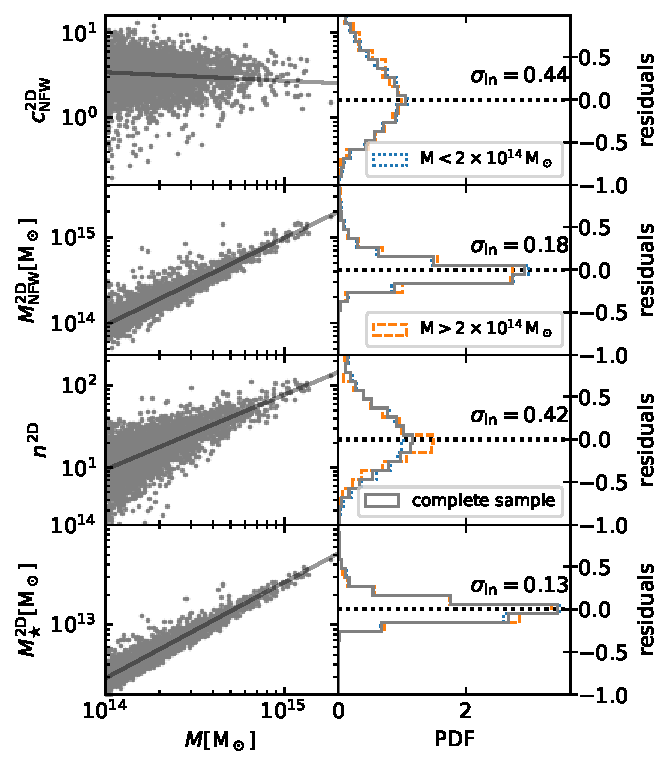
\includegraphics[width=\linewidth]{figure/mass_eucl.pdf}\\
\caption[h]{Magneticum mass-observable relation for \Euclid-like derived quantities. Left column shows scaling relations and relative fit. Right column shows the residual PDF and scatter of log-residuals $\sigma_{\rm ln}.$ We report the following properties: lensing concentration $c^{\rm 2D}_{\rm NFW}$ (first row), lensing mass  $M^{\rm 2D}_{\rm NFW}$ (second row), projected  richness $n^{\rm 2D}$ (third row),  and projected stellar mass $M_\star^{\rm 2D}$ (fourth row).   The histogram of residuals for haloes with $M<2\times10^{14}\,{\rm M}_\odot$ is in blue dotted lines, for   haloes with $M>2\times10^{14}\,{\rm M}_\odot$ is in orange dashed lines, and for the complete sample is in solid grey lines. Note that the three histograms almost overlap. Each distribution panel reports the value of the natural log scatter $\sigma_{\rm ln}$ for the complete sample.
%We over-plot observations from \cite{2006ApJ...640..691Vikhlinin}, \cite{2009ApJ...693.1142Sun}, \cite{2018ApJ...867...12Rettura} for richness from X-ray and SZ selections,and the stellar masses compared to the work of ~\cite{2013ApJ...778...14Gonzalez}.   
}
\label{fig:compare_obs_eucl}
\end{figure}

\begin{figure}
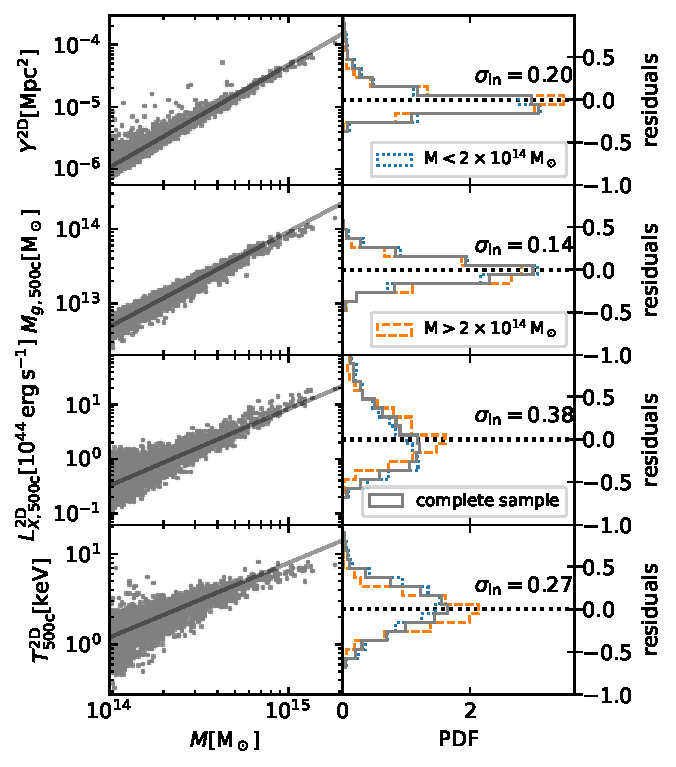
\includegraphics[width=\linewidth]{figure/mass_mwl.pdf}\\
\caption[h]{As Fig.\,\ref{fig:compare_obs_eucl}, but for the following multi-wavelength observable properties: projected integrated Compton-$y$ parameter $Y^{\rm 2D}$ (first row),  the  3D gas mass $M_{\rm g, 500c}$ (second row), the projected X-ray luminosity in the soft band (in range $[0.5,2]\,{\rm keV}$) $L^{\rm 2D}_{\rm X, 500c}$ (third row),    and  the projected temperature $T^{\rm 2D}_{\rm 500c}$ (fourth row). The values of X-ray luminosity, gas mass, and temperatures are reported within an overdensity of $r_{\rm 500c}$ as this definition is a typical choice in X-ray based observations.
}
\label{fig:compare_obs_oth}
\end{figure}


In  Fig.\,\ref{fig:compare_obs_eucl} we show the observable properties vs. true mass $M$ of clusters, derived from Magneticum Box2b/hr simulation for  properties that could be derived by \Euclid data, as lensing concentration (first row), lensing mass (second row), projected  richness (third row), and projected stellar mass (last row), as presented in Sect.~\ref{sec:obs}.
For each property we fit a scaling relation performed using a linear regression in the log-log space.  In the right panel of Fig.\,\ref{fig:compare_obs_eucl},   we show the log-residual distribution  for both low mass haloes ($M<2\times10^{14}\,{\rm M}_\odot$), high mass haloes ($M>2\times10^{14}\,{\rm M}_\odot$), and  for the complete sample of the log-residuals $\sigma_{{\rm ln},i}$, defined as the natural logarithmic ratio between the $i-$th cluster property and the corresponding scaling relation value at its mass.
 In the second column we also report the log-scatter  $\sigma_{\rm ln}$ defined here as the corresponding standard deviation of the log-residual, namely
 \begin{equation}
 \sigma_{\rm ln}\left[X\right] = \operatorname{E}\left[\left(\sigma_{{\rm ln},i} - \operatorname{E}\left[\sigma_{{\rm ln},i}\right]\right)^2\right]^{1/2},    
 \label{eq:sigmaln}
 \end{equation}
 %
 where $\operatorname{E}$ is the expectation operator.
 We note that the concentration has a scatter of $0.47$ which is higher than theoretical expectations~\citep[see e.g.,][]{Child2018MCscatter}.
 Throughout this paper we will show that this is due to projection effects, in fact, the 3D concentration has a scatter of $\approx0.33.$
 We also note that the mass-concentration relation is relatively flat compared to dark matter only simulations~\citep{Duffy08Mc} in agreement with the fact that hydrodynamic simulations tend to have flatter mass-concentration relation, see for instance green data points in Fig. 8 of ~\cite{2010MNRAS.405.2161Duffy}.



 In Fig.\,\ref{fig:compare_obs_oth} we show the mass-observable relations  of  quantities that could potentially be obtained from various multi-wavelength observations that could enrich studies based on \Euclid data products:  the integrated Compton-$y$ parameter, the gas mass $M_{\rm g,500c}$,   the X-ray luminosity $L_{\rm X,500c}^{\rm 2D}$ converted in the soft band $[0.5,2]\,{\rm keV},$ and the  temperature $T_{\rm 500c}.$
 We decided to plot the X-ray luminosity, gas mass and temperature within $r_{\rm 500c}$  because this radius is typically used in various X-ray observations~\cite[see e.g.,][]{2006ApJ...640..691Vikhlinin,2009ApJ...693.1142Sun}.
 Note that we plot the gas mass in 3D (instead of the projected gas mass) because hydrostatic mass as derived from X-ray observations is closer to the 3D one rather than the projected one~\citep{Ettori2013MassProfiles}.




\section{Projection effects}
\label{sec:proj}

\begin{figure*}
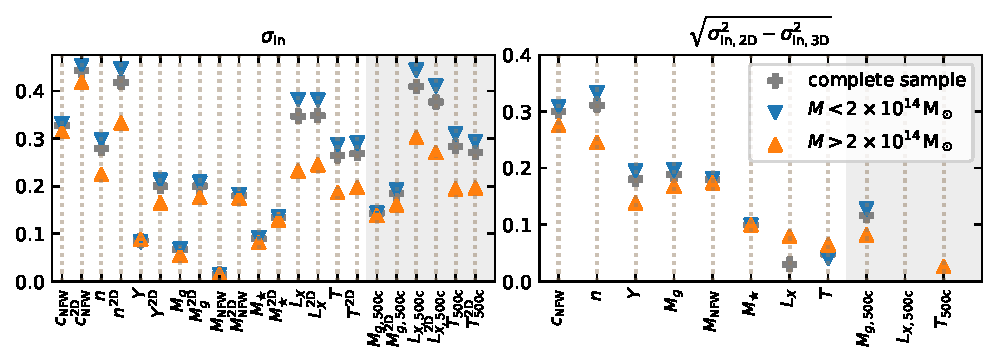
\includegraphics[width=\linewidth]
{figure/sigma.pdf}
\caption[h]{Scatter of our mass-observable relations: concentration, richness, integrated Compton-$y$ parameter, gas mass, NFW mass,  stellar mass,  X-ray luminosity, and temperature, within a radius of $r_{\rm 200c},$ and grey band report the gas mass, X-ray luminosity, and temperature within $r_{\rm 500c}.$ 
Left panel reports the fractional scatter of both 3D and 2D quantities.
Right panel reports the contribution of projection effects.
Points are coloured by their mass range as in Fig.\,\ref{fig:compare_obs_eucl}, blue down-triangles represent the low mass bin, orange up-triangles represent the high mass bin, and grey crosses represent the complete sample.
Note that we lack the value of projection effects for $L_{\rm X, 500c}$ (see discussion). Points are ordered according to their value of the second panel. Error bars are on the first and third panels are computed using jackknife method. }
\label{fig:sigma}
\end{figure*}

\begin{figure}
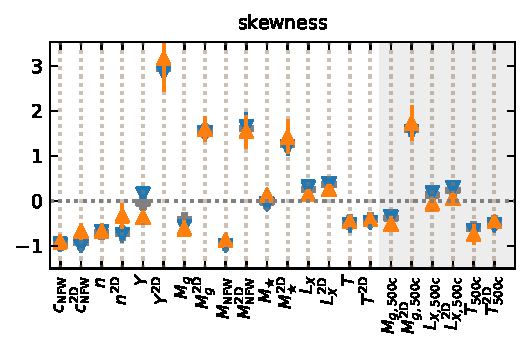
\includegraphics[width=\linewidth]
{figure/skew.pdf}
\caption[h]{Skewness parameters  for our cluster properties. Data, line styles and colours are as in Fig.\,\ref{fig:sigma}. }
\label{fig:skew}
\end{figure}


\begin{figure}
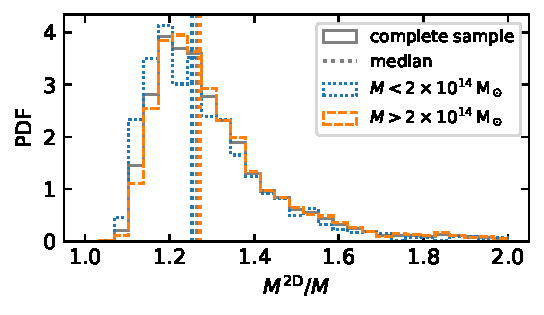
\includegraphics[width=0.9\linewidth]{figure/M2D_M_pdf.pdf}
\caption[h]{Probability density distribution of $M^{2D}/M$ at different mass bins:  for haloes with $M<10^{14}\,{\rm M}_\odot$ as a blue dotted line,  for   haloes with $M>10^{14}\,{\rm M}_\odot$ as a dashed orange line and for the complete sample as a gray solid line. For each mass bin we report a vertical line with the median values (note that the three lines are very close together).}
\label{fig:M2DPDF}
\end{figure}

\begin{figure*}
\begin{subfigure}[b]{0.01\linewidth} % Adjust the width as needed
        \rotatebox[origin=l]{90}{\hspace{1.5cm}{\tiny{$23\,{\rm Mpc}$}}}
    \end{subfigure}
    \hfill
    \begin{subfigure}[b]{0.98\linewidth} % Adjust the width as needed
        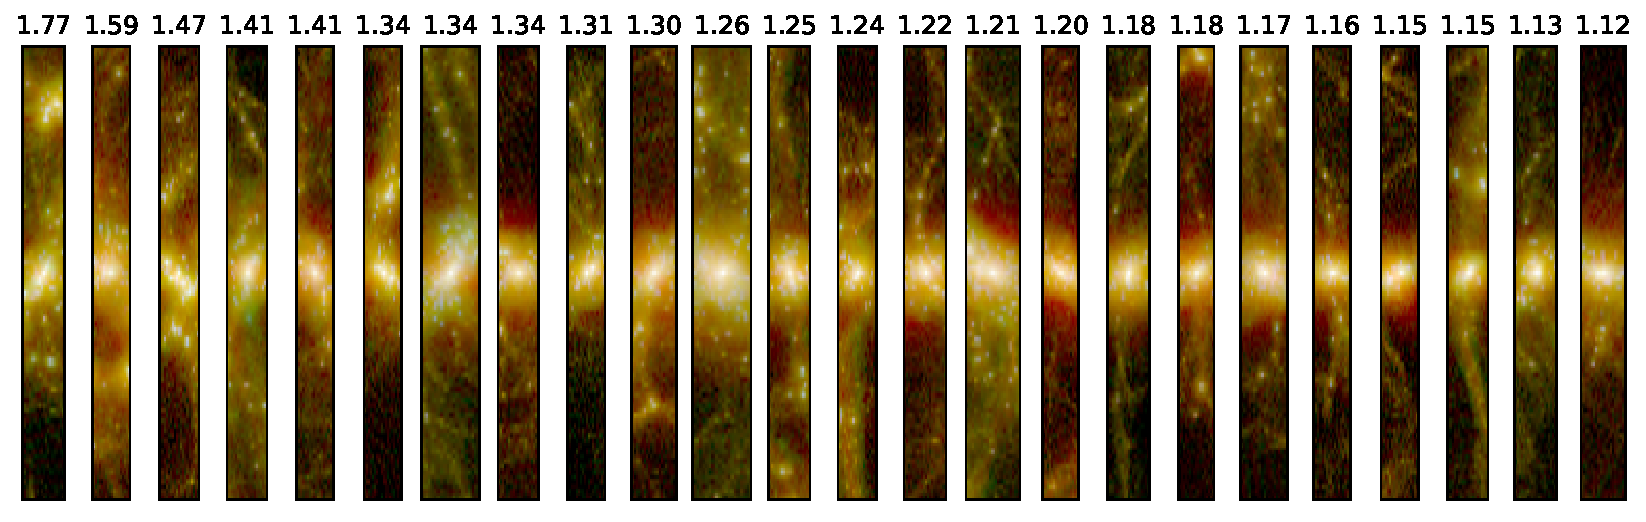
\includegraphics[width=\linewidth]{figure/map_random.pdf}
    \end{subfigure}
\caption[h]{Projected maps along a  cylinder of length $23\,{\rm Mpc},$ with radius $r_{\rm 200c}$  and centred on a random sample of our galaxy clusters, ordered by their  $M^{\rm 2D}/M$ (over-plotted above each map) values decreasing from left to right. The red band maps the gas projected mass, the green band maps the dark matter projected mass and the blue band maps the stellar projected mass. }
\label{fig:map_random}
\end{figure*}


\begin{figure*}
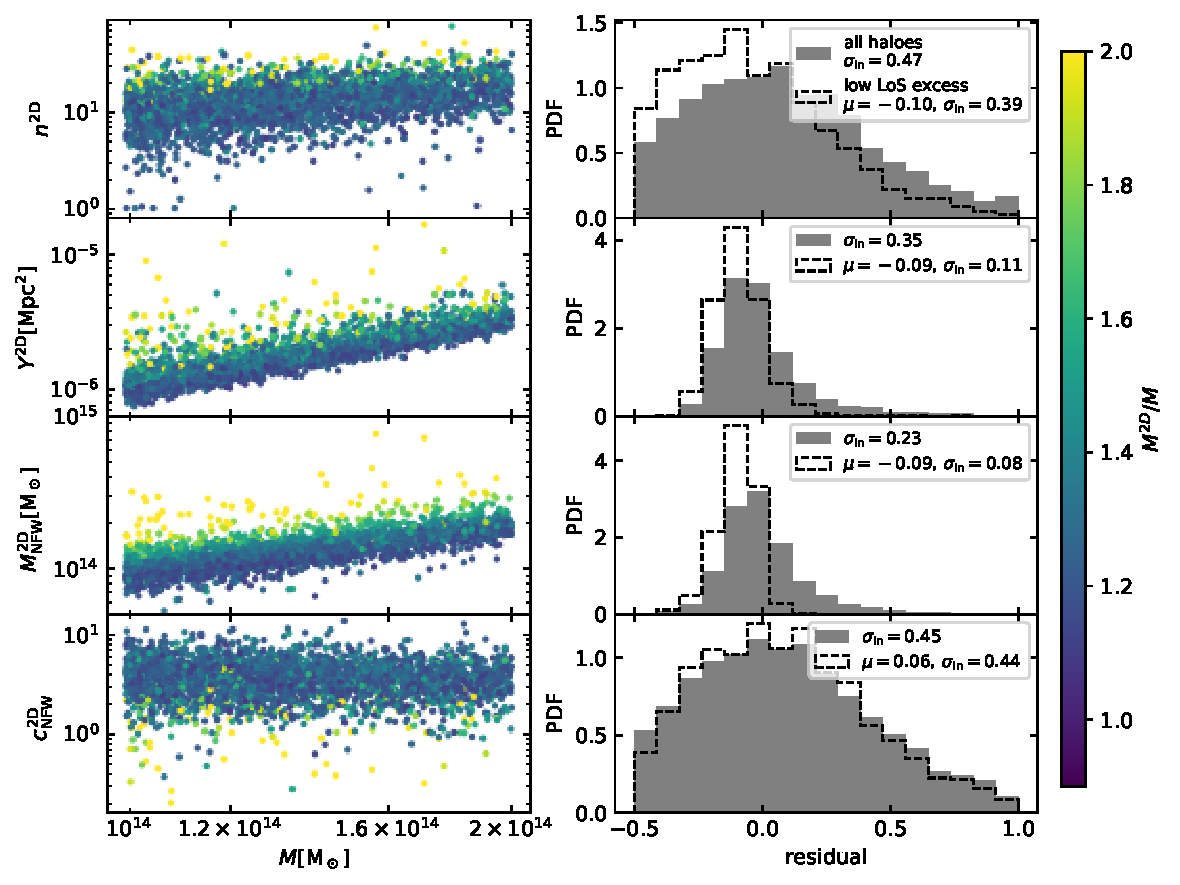
\includegraphics[width=\linewidth]{figure/residuals_2d.pdf}
\caption[h]{Impact of LoS contamination in scaling relations. We show halo properties  as a function of halo mass $M$
in the left column, and colour coded by  fractional amount of mass in cylinder ($M^{\rm 2D}/M$), and the residuals PDFs in the right column (grey shaded histogram).
Rows correspond to: richness, the integrated Compton-$y$ parameter, lensing mass and lensing concentration. We also show the residuals of a subset of haloes with low LoS contamination (in particular $M^{\rm 2D}/M<1.26,$ dashed line histogram). Each panel reports the scatter of the  residuals $\sigma$, and the mean $\mu$ of the low LoS residuals. }
\label{fig:residuals_2d}
\end{figure*}

\begin{figure}
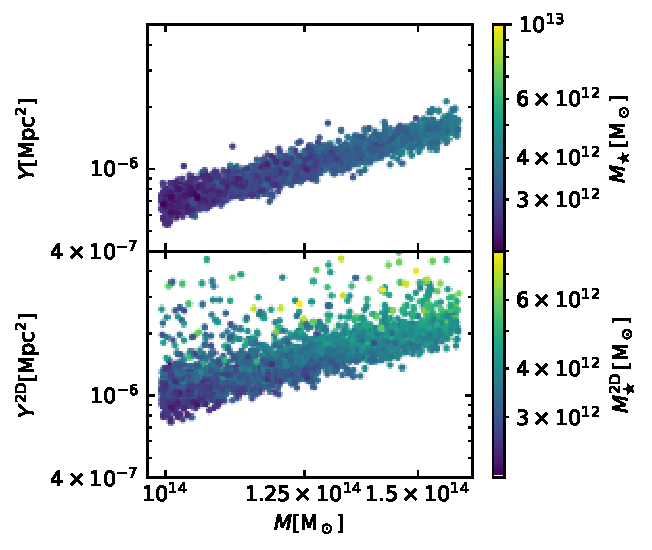
\includegraphics[width=\linewidth]{figure/3d_vs_2d.pdf}
\caption[h]{integrated Compton-$y$ parameter vs. halo mass, color coded by stellar mass fraction. Top panel shows quantities as computed within a sphere of radius $r_{\rm 200c}$, while on the bottom panel they are computed within a cylinder (of radius $r_{\rm 200c}$ and length $20\,{\rm Mpc}$ as already presented in Sect. \ref{sec:setup}).}
\label{fig:3d_vs_2d}
\end{figure}


The main objective of this work is to disentangle the amount of scatter and skewness in scaling relations that is purely due to projection effects.
Note that  observational data are also affected by measurement errors that we cannot tackle in this work. 
In this Sect. we quantify the scatter and skewness of mass-observable relations and asses the impact of projection effects at low redshift ($z=0.24$) as we have a larger sample of galaxy clusters and spanning a wide range of masses, we will present the scatter and skewness at high redshift  ($z=0.9$) in Sect.~\ref{sec:z1}.

To asses the role of projection effects, in  Fig.\,\ref{fig:sigma} we report the 3D and 2D scatter of our cluster properties.
In the left panel of Fig.\,\ref{fig:sigma} we show 
the value of the scatter of log-residuals $\sigma_{\rm ln}$ for all our mass-observable relations.
In the shaded region we also report the values computed within $r_{\rm 500c}$ for the X-ray luminosity, gas mass, and temperature values, because this is the overdensity that is typically used in X-ray analyses.

For each  observable, in Fig.\,\ref{fig:sigma} we report both the scatter of the complete sample as well as the one of two smaller mass bins  ($10^{14}<M<2\times10^{14}\, {\rm M}_\odot$ and $M>2\times10^{14}\, {\rm M}_\odot$).
We note that the lower mass bin ($M<2\times10^{14}\, {\rm M}_\odot$) is the one with largest scatter, because for a given external object in the line-of-sight (LoS), the profile of a small cluster will be perturbed more with respect to a massive cluster. 

  In the left panel of Fig.\,\ref{fig:sigma} we see  that  some quantities have a low scatter in the 3D space and do gain a large amount of scatter once they are seen in projected space. 
To quantify better what is the actual impact of projection effects, in the right panel of Fig.\,\ref{fig:sigma} we present the metric $\sqrt{\sigma_{\rm ln, 2D}^2 - \sigma_{\rm ln, 3D}^2}.$ 
This metric shows that the quantities that are most affected by projection effects are the weak lensing concentration, integrated Compton-$y$ parameter, the richness, the NFW lensing mass, and the gas mass.
We note that the scatter in the richness is relatively higher than other theoretical predictions~\citep[see e.g.][]{Castignani2016richness}, and we anticipate that this happens only at this low-redshift slice and our projected richness at $z=0.9$ has a scatter of log-residuals of $0.31$ (see Sect.~\ref{sec:z1}).

We note that X-ray luminosity and temperature are the least impacted by effects from projections,
the reason is that X-ray luminosity depends on gas density squared and thus only affected by the most peaky regions in an image, and that temperature is mostly affected by the most internal part of a cluster.
Note that we lack the value of projection effects for $L_{\rm X, 500c}$ because the 2D scatter is slightly smaller than the 3D one. This happened because projection effects impact under-luminous haloes more strongly than overly-luminous haloes (at a fixed mass bin), with the consequence of the projected X-ray luminosity having a higher normalisation and a lower scatter (see Fig. ~\ref{fig:LX3D_vs_2D}).


We also quantify deviations of residuals from a symmetrical distribution  by introducing  the  the Fisher-Pearson coefficient  of skewness ${m_3}/{m_2^{3/2}},$ where $m_k$ is the sample  $k$th  central moment.\footnote{
 Where the central moment $m_k$ for a random variable $X$ is defined as $\operatorname{E}\left[ ( X - \operatorname{E[X]})^n \right].$
}
We report its dependency on projection effects in  Fig.\,\ref{fig:skew}, where we can see that the properties whose skewness is most impacted by projection effects are the gas mass, the integrated Compton-$y$ parameter, and the lensing NFW mass.
{ We also notice that some scaling relation residuals move from having a negative skewness (for the NFW concentration for instance, due to un-relaxed and merging clusters) to a positive one once projection effects are taken into account.
}




To assess the impact of projection effects we introduce a variable to quantify the amount of additional matter in the line of sight   that can skew our observable properties. We define it as the ratio of the mass within the cylinder and the mass within a sphere $\mrat,$ both of radius $r_{\rm 200c},$ and the length of the cylinder are described in Sect. \ref{sec:setup}.
We present the distribution of $\mrat$ in Fig.\,\ref{fig:M2DPDF}, where we can see that this quantity is strongly skewed and its median value is $M^{\rm 2D}/M\approx1.26$ (we stress that the aperture radii are $r_{\rm 200c}$).
Although this quantity is not directly observable, we will use it to asses the contribution of LoS objects in projection effects. Note that besides objects in the LoS, also different fitting procedures may impact the scatter of projection effects, as we will see in Sect. \ref{sec:MC}.


In Fig.\,\ref{fig:map_random} we show a random selection of clusters, ordered by  $\mrat$  from left to right.
Objects with high $\mrat$ (the objects in the left-most panels) include clusters that are merging, elongated or in the LoS, in the rest of this paper we will refer to the objects as having $\mrat$ greater than the median of the distribution $1.26$ as having LoS  excesses.


To study the impact of projection effects in scaling relations, in Fig.\,\ref{fig:residuals_2d} we show the scaling relations of the following projected quantities: richness, integrated Compton-$y$ parameter, lensing mass and concentrations, that are the ones that are most affected by projection effects.
We colour-code these points by   $\mrat$ and focus on a narrow mass range of $M\in[1,2]\times10^{14}\,{\rm M}_\odot$ in order to visualise better how LoS excesses impact these scaling relations.
On the left column we can visually see that, except for concentration, they strongly correlate with $\mrat,$ as the upper points of the scatter plot tend to have higher values of $\mrat.$
 
We quantify this finding in  the right column by 
comparing the residual distributions (of the power law fit over the complete mass range presented in Sect.~\ref{sec:cumpa}) of the complete sample with the distribution of objects with low LoS contamination only (we adopt the criteria of $\mrat<1.26$ as being the median of the $\mrat$ distribution, as shown in Fig.\,\ref{fig:M2DPDF}),  and report the respective scatter $\sigma$ and average value $\mu$ of the residual distributions (for the complete sample we have that $\mu=0$).
Except for the concentration, residuals of haloes with low $\mrat$ (see dashed histogram),  are significantly shifted towards negative values of $\mu$ and $\sigma.$
For instance, the scatter of $Y^{\rm 2D}$ decreases from $0.35$ down to $0.11$ when we consider only objects with a low LoS excess. 

It is interesting that although concentration from weak lensing signal is heavily impacted by projection effects (it is the quantity with the highest scatter in Fig.\,\ref{fig:sigma}), its scatter is not dominated by objects in the LoS (projection effects here denote all consequences of measuring a quantity in projection: LoS effects as well as fitting procedures).
We devote the next section in showing that the reason for concentration being strongly affected by projection effects is that their reduced shear profile deviates strongly from the one coming from NFW profiles~\citep[see e.g.,][]{2021MNRAS.500.5056Ragagnin} which is used to reconstruct the reduced shear profile. 


To conclude this section, we now study how correlations between cluster observable properties can be affected by projection effects.
To this end we take the case of a possible hot- vs. cold-baryon correlation by studying the stellar mass vs. integrated Compton-$y$ parameter (as the latter should strongly correlate with the gas mass).
In Fig.\,\ref{fig:3d_vs_2d} we show the integrated Compton-$y$ parameter scaling relation,   colour coded by stellar mass  for the 3D quantities (top panel) and projected quantities (bottom panel).  If we look at the correlations at a fixed mass between our quantities as computed into spheres (top panel in Fig.  \ref{fig:3d_vs_2d}) then we can  see a weak anti-correlation between stellar mass and the integrated Compton-$y$ parameter (we quantify it in Sect. \ref{sec:cova}) in agreement with the fact that for a fixed baryon fraction, a larger stellar fraction implies a lower gas fraction,
while if we look at the properties in the projected space, they show a stronger correlation. This implies that projection effects can be so relevant to produce a correlation between observable properties.
While this analysis is purely qualitative, we will quantify the impact of this projection effects in Sect.~\ref{sec:cova}, where we will compute both the correlation coefficients for both 3D quantities and 2D quantities.

\section{Projection effects on lensing concentration}
\label{sec:MC}

\begin{figure}
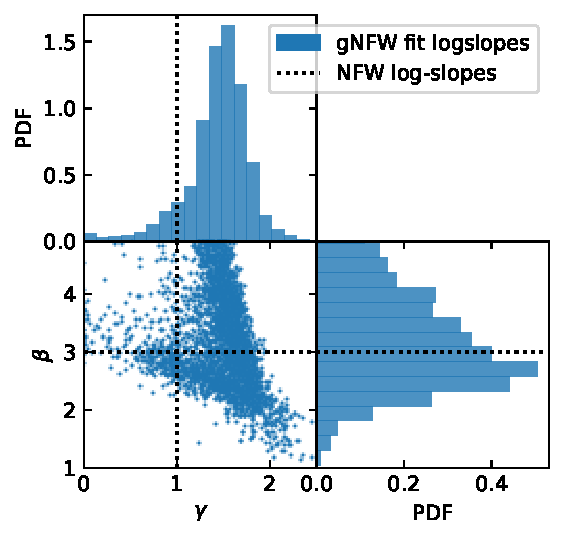
\includegraphics[width=\linewidth]{figure/gamma_beta.pdf}
\caption[h]{Probability density distribution of the parameters $\gamma$ (inner slope, upper panel) and $\beta$ (outer slope, right panel) of Eq. \eqref{eq:gnfw} of the successful gNFW fits. Central panel shows the scatter plot between the two parameters. The dotted lines shows the NFW parameters $\gamma=1$ and $\beta=3.$}
\label{fig:gamma_beta}
\end{figure}

\begin{figure}
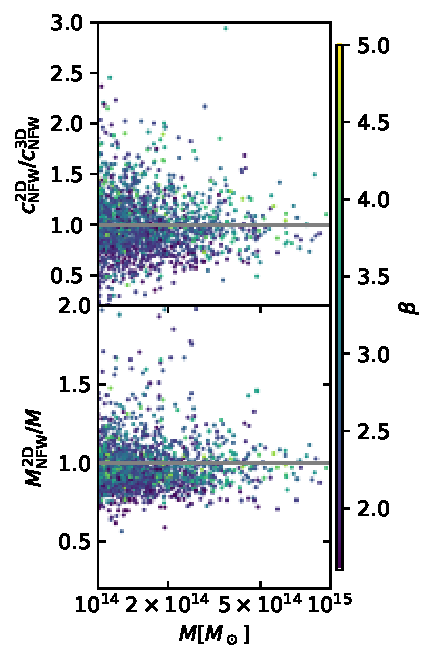
\includegraphics[width=0.95\linewidth]{figure/Mcs.pdf}
\caption[h]{Ratio between 2D NFW fit parameters and 3D parameters for haloes with a successful 3D gNFW fit.
Upper panel: ratio between concentrations; lower panel: ratio between halo masses.
Points are colour-coded by the external log slope $\beta$ of the 3D fit of gNFW.   }
\label{fig:c_ratios}
\end{figure}



\begin{figure}
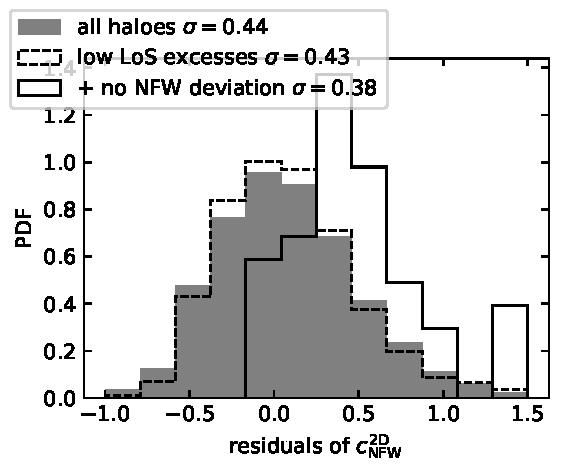
\includegraphics[width=0.9\linewidth]{figure/residuals_c.pdf}
\caption[h]{Residuals of lensing concentrations with respect to the power law fit. As in Fig.\,\ref{fig:residuals_2d}, the dashed line histogram indicates the residuals for objects with low LoS effects (low low value of $\mrat$).  
Solid line histograms contains the additional constrain of haloes having high NFWness ($2.8<\beta<3.2$ and $0.8<\gamma<1.2$). Each histogram reports the scatter $\sigma$ of the residuals.}
\label{fig:residuals_2d_mc}
\end{figure}


\begin{figure}
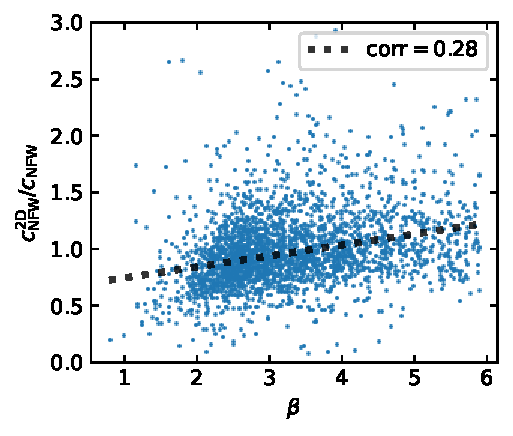
\includegraphics[width=0.9\linewidth]{figure/c_ratio_vs_beta_corr.pdf}
\caption[h]{Scatter plot of ratio between 2D concentration and 3D concentration against $\beta,$ namely the outer slope of Eq. \eqref{eq:gnfw}, of well behaving 3D gNFW fits in a narrow mass range of $M\in[1,2]\times10^{14}\,{\rm M}_\odot.$ We also report the correlation coefficient.}
\label{fig:c_ratio_beta}
\end{figure}


As we found in the previous section,  projection effects significantly increase the scatter and skewness in the scaling of lensing concentration with mass.
However, the scatter increase does not seem to be related to external objects in the LoS, and now we assess if the high scatter of lensing concentration is due to deviations of the reduced shear profile from the one induced by an NFW profile. 
In this work we will not investigate the origin of this deviation as it is out of the scope of this paper.
Such deviation may arise from halo elongations or the fact that NFW profile does not describe the density profile of galaxy clusters (from hydrodynamic simulations) up to the accuracy we need here. For instance there are hints that a truncated NFW profile may suite galaxy clusters better~\citep{Oguri+2011truncatedNFW}.


To study deviations  from the NFW profile of haloes we fit a generalised NFW profile~\citep{Nagai2007gNFW}, hereafter gNFW, in spherical coordinates over the same radial range as our previous NFW profile (described in Sect. \ref{sec:obs}), where the density profile  $\rho_{\rm gNFW}\left( r \right)$ is defined as
%
\begin{equation}
\rho_{\rm gNFW}\left( r \right) = \frac{\rho_0}{\left(r/r_{\rm s}\right)^\gamma\left(1+r/r_{\rm s}\right)^{\beta-\gamma}},
\label{eq:gnfw}
\end{equation}
%
where $\gamma$ and $\beta$ are respectively the internal and external log slopes of the total matter density profiles.
Note that \cite{Nagai2007gNFW} gNFW also depends on the  parameter $\alpha$ that  we fix to $\alpha=1$ for this work.
Note that for $\gamma=1$ and $\beta=3$ one recovers the NFW profile as in Eq. \eqref{eq:nfw}.
We present the PDF of the 3D fit of the gNFW profile parameters  $\gamma$ and $\beta$ distribution in Fig.\,\ref{fig:gamma_beta}, where the fit was performed with a bound of $\gamma\in[0,3]$ and $\beta\in[0,6]$. We observed that the fitting procedure yielded successful results for approximately 3500 objects, constituting a subset of the total 4300 objects. These objects exhibited values for $\gamma$ and $\beta$ below the upper limit of the specified interval. We have excluded these particular haloes from the analyses presented in this section. Upon visual inspection, these excluded objects displayed a sharp decline in the outskirts of the matter density profile, resembling a truncated NFW profile. While it could be argued that a truncated NFW fit might be more suitable for this analysis, our objective is to investigate the effects of deviations from the NFW profile. Therefore, the choice of a generalized NFW (gNFW) fit is more fitting for our study.


In Fig.\,\ref{fig:c_ratios}, we plot the values of concentration and mass obtained from reduced shear fit, divided by the corresponding 3D quantities and colour-coded by the external 3D gNFW slope $\beta$ for our intermediate redshift haloes. 
As we can see,  haloes with large values of $\beta$ have a lensing concentration that is significantly higher than the 3D one (see upper panel).
In Appendix \ref{ap:gnfw} we report the example of a simulated halo with low LoS excess (see Fig.\,\ref{fig:example}) and an analytical one (see Fig.\,\ref{fig:colossus}), both with a flat external log-slope, and we show how the under-estimation of the concentration is caused by the fact that the NFW fit on the reduced shear is weighting too much the external part of the profile, that deviates from an NFW.
In Fig.\,\ref{fig:residuals_2d_mc}, we show the concentration  residual distribution and report their scatter.
We show that if one excludes objects with strong LoS contribution, the large scatter of the lensing concentration is not affected.
However if one also restrict our sample to objects having NFW-like external log-slopes (we used a criteria of $2.8<\beta<3.2$ and $0.8<\gamma<1.2$) then the scatter of concentration residuals decreases drastically from $0.45$ to $0.39.$
We also show how the external log-slope of the halo profile affects the lensing reconstruction by plotting the ratio between the projected and 3D concentration (i.e. $c^{\rm 2D}_{\rm NFW}/c_{\rm NFW}$) value versus the 3D log-slope $\beta$ in the narrow mass bin of $M\in[1,2]\times10^{14}\,{\rm M}_\odot$ in Fig. ~\ref{fig:c_ratio_beta}, where we find a positive correlation coefficient of $\approx0.28.$




\section{Correlations between properties}
\label{sec:cova}

\begin{figure*}
{\centering 
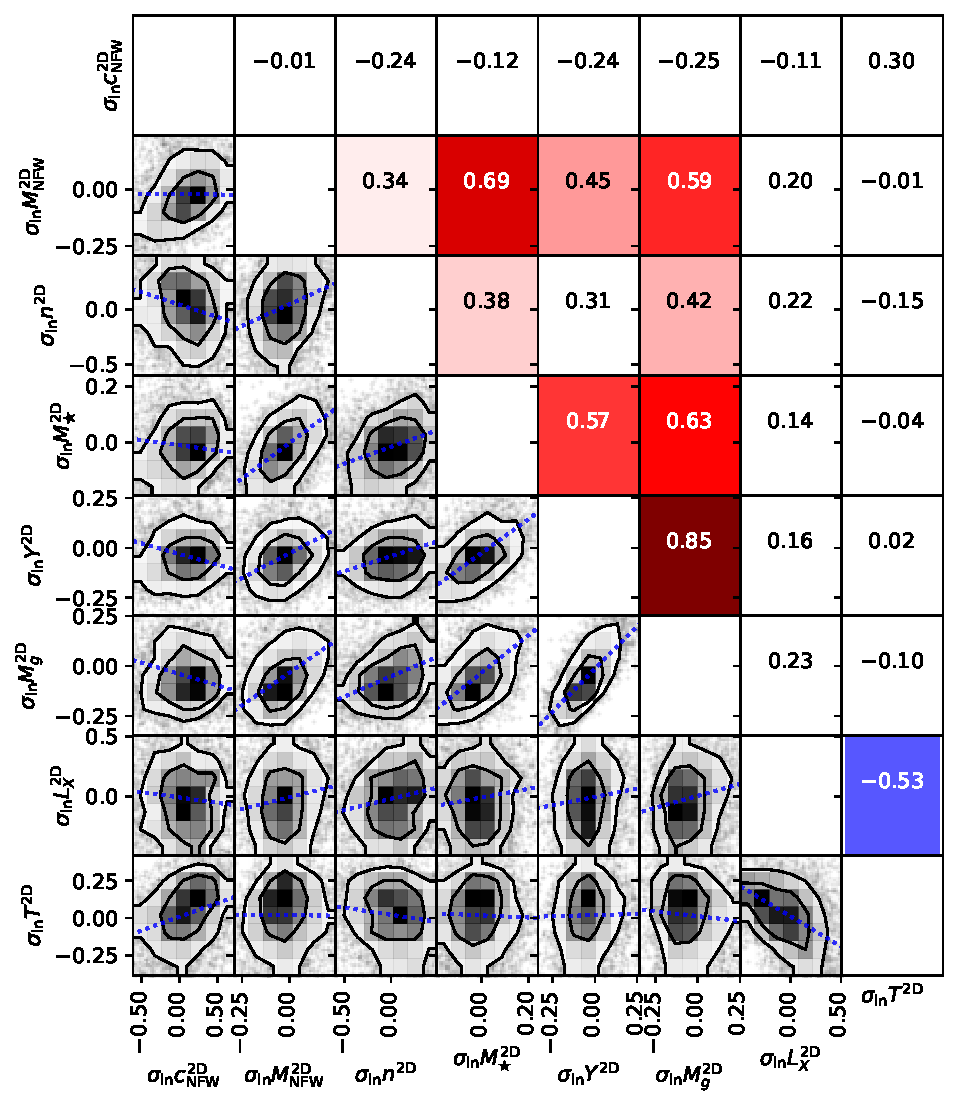
\includegraphics[width=0.95\linewidth]{figure/covarma-2D.pdf}
}
\caption[h]{Correlation coefficients matrix (upper-right triangle) and scatter plot (bottom-left triangle) of power-law log-residuals  of \Euclid data (lensing concentration, lensing mass, richness, and stellar mass, respectively) and possible outcomes from multi-wavelength observations (integrated Compton-$y$ parameter, gas mass, X-ray luminosity and temperature respectively).} 
\label{fig:covarma2D}
\end{figure*}



\begin{figure*}
{\centering 
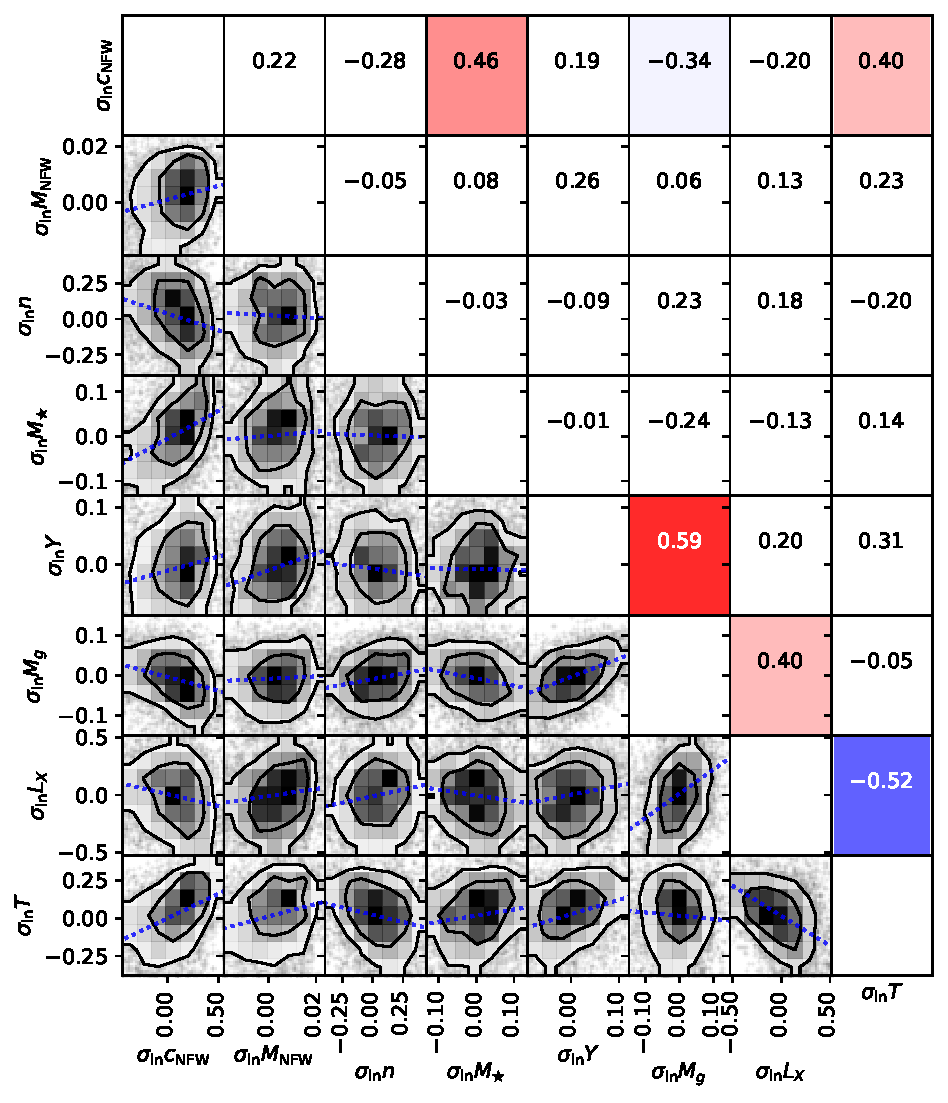
\includegraphics[width=0.95\linewidth]{figure/covarma-3D.pdf}
}
\caption[h]{As Fig.\,\ref{fig:covarma2D}, here we show the quantities computed in the 3D space.}
\label{fig:covarma3D}
\end{figure*}

\begin{figure*}
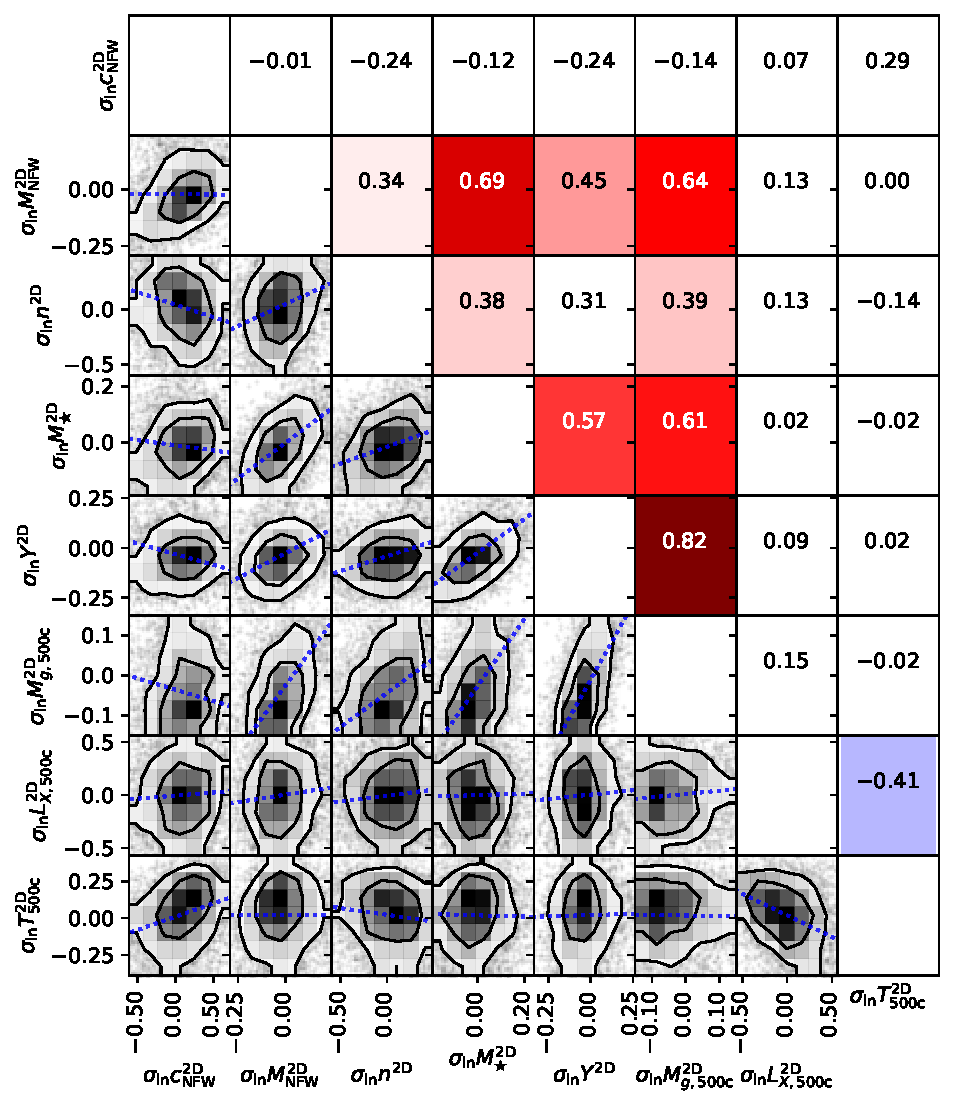
\includegraphics[width=\linewidth]{figure/covarma-2D-500c.pdf}
\caption[h]{As Fig.\,\ref{fig:covarma2D},  but we show the projected X-ray luminosity, the projected gas mass, and the projected temperature computed within the overdensity of $\Delta={\rm 500c}$ instead of the respective quantities within $\Delta={\rm 200c}.$}
\label{fig:covarma2D500c}
\end{figure*}



\iffalse
\begin{figure*}
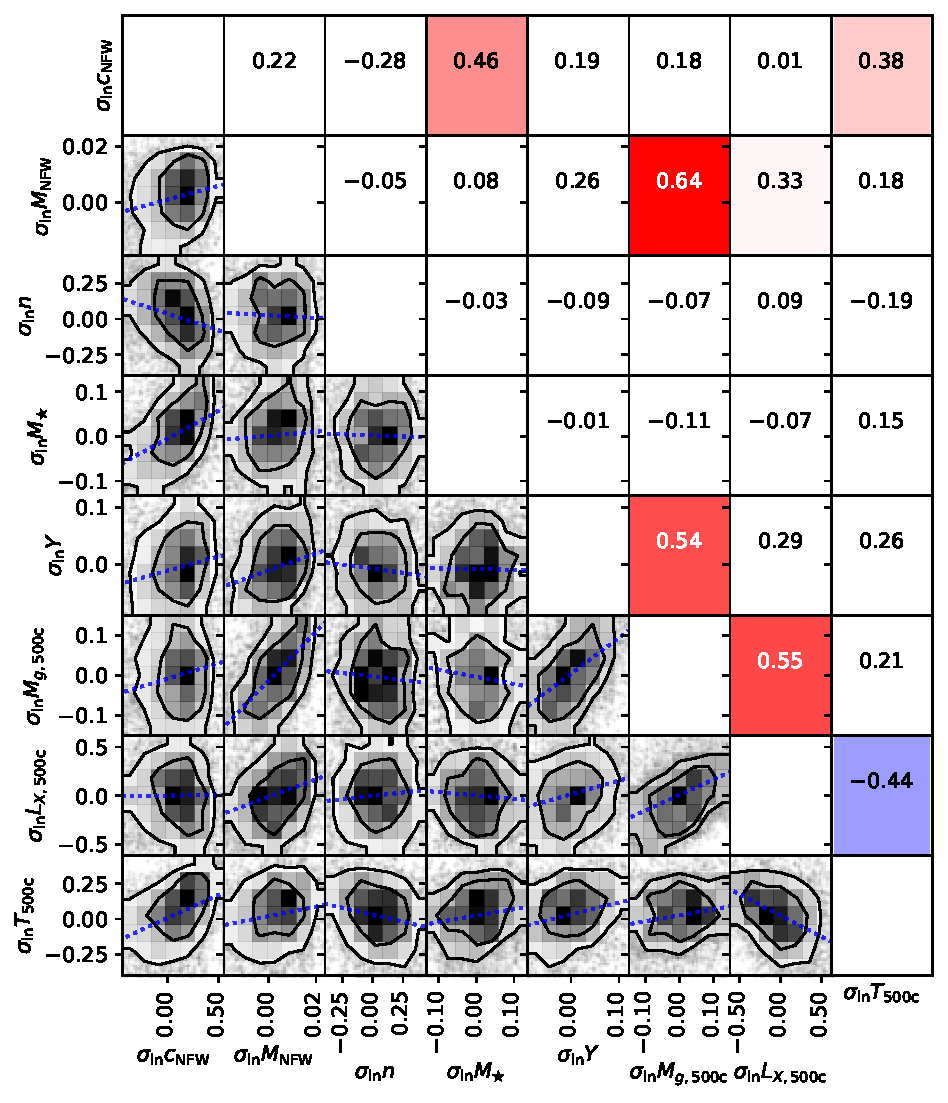
\includegraphics[width=\linewidth]{figure/covarma-3D-500c.pdf}
\caption[h]{As Fig.\,\ref{fig:covarma3D},  but we present the 3D X-ray luminosity, the 3D gas mass, and the 3D temperature computed within the overdensity of $\Delta={\rm 500c}$ instead of the respective quantities within $\Delta={\rm 200c}.$}
\label{fig:covarma3D500c}
\end{figure*}
\fi

While in the last sections we investigated the origin the impact of projection effects in the scatter and skewness of observable properties, we will now quantify how projection effects do impact the correlation between observable properties.
We quantify the correlation coefficients computing the Pearson coefficients between residuals of their log-log scaling mass-relations.

In Fig.\,\ref{fig:covarma2D} we show the correlation coefficient matrix  between log-residuals at fixed halo mass of our projected observable both from \Euclid data (lensing concentration, lensing mass, richness and stellar mass, respectively) and possible outcomes from multi-wavelength observations (integrated Compton-$y$ parameter, gas mass, X-ray luminosity and temperature) for intermediate redshift objects. 

We note  that concentration anti-correlates with gas-mass (and integrated Compton-$y$) parameter, in agreement with other theoretical data such as ~\cite{2022A&A...666A..22Ragagnin}.
Moreover, at fixed halo mass, the lensing mass correlates strongly with total projected stellar mass and projected gas mass, which may be due to the fact that both correlates strongly with LoS contamination. 
The same is true for the strong  correlation between richness, gas mass and stellar mass, because projection effects makes so that a LoS excess will boost all these quantities (as noted in the Sect. \ref{sec:cumpa}). 
We note that the 2D lensing mass and projected X-ray luminosity  have a slight  positive correlation, in agreement with the observational work of ~\cite{2020MNRAS.492.4528Sereno}.

In Fig.\,\ref{fig:covarma3D} we show the covariance matrix of non-projected quantities  for intermediate redshift objects.  
We see that opposed to Fig.  ~\ref{fig:covarma2D}, the 3D covariance matrix shows a mild yet negative covariance between gas mass and stellar mass, and a 
much lower correlation between richness and gas mass, because most of their correlations in the projection is due to LoS excesses that significantly increase the values of the gas mass, the richness and the stellar mass.
In Fig.\,\ref{fig:covarma2D500c}  we report the correlation matrix as Fig.\,\ref{fig:covarma2D} and Fig.\,\ref{fig:covarma3D} respectively where we present X-ray luminosity, gas mass, and temperature, 
as computed within $r_{\rm 500c},$ which produce a positive correlation coefficients between the gas mass and the concentration  (while in Fig.\,\ref{fig:covarma3D} we have seen that they do anti-correlate).
One possibility is that this  change in sign of the correlation is caused by the fact that mixing overdensities (concentration is within $\Delta_{\rm c}= 200$ and gas-mass is within  $\Delta_{\rm c}= 500$) does introduce an additional correlation with the sparsity~\citep{Balmes2014Sparsity,Corasaniti2022Sparsity} that itself correlates with the concentration (see Appendix \ref{ap:500}).

 For completeness we report the correlation coefficient matrix and the scatter of log-residuals of all quantities in Table~\ref{table:z0}.
 There we also added the core-excised projected X-ray luminosity $L_{\rm X,ce500c}^{\rm 2D}$, as it is often used in X-ray based observational studies, where we can see that the scatter and most of correlation coefficients are smaller than $L_{\rm ce500c}^{\rm 2D},$ while the correlation with the concentration and gas mass increase.
 Note that we do not report the 3D NFW mass ($M_{\rm NFW}$) because it has an extremely low intrinsic scatter $\sigma_{\rm ln} \left(M_{\rm NFW}\right)\approx0.01$ and its correlation coefficients are not meaningful.


\subsection{Analysis at $z=0.9$}
\label{sec:z1}

\begin{figure*}
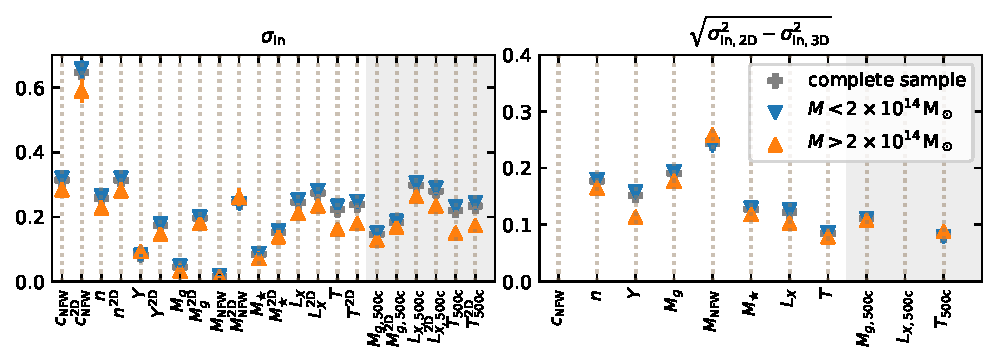
\includegraphics[width=\linewidth]{figure/sigmaz1.pdf}
\caption[h]{Same as Fig.\,\ref{fig:sigma} for the data at $z=0.9.$ We do not report the value fo the concentration because in our fit radial range the lensing one does not correlate with the 3D one.}
\label{fig:sigmaz1}
\end{figure*}

\begin{figure}
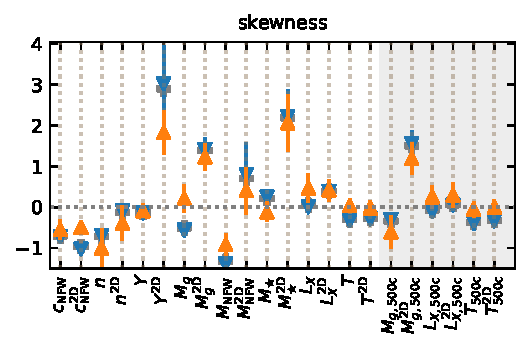
\includegraphics[width=\linewidth]{figure/skewz1.pdf}
\caption[h]{Same as Fig.\,\ref{fig:skew} for the data at $z=0.9.$ We do not report the value fo the concentration because in our fit radial range the lensing one does not correlate with the 3D one.}
\label{fig:skewz1}
\end{figure}


In this section we present the correlation coefficients and covariance matrices at $z=0.9.$
It is interesting to study this redshift slice because it is still of interest for the \Euclid mission, and both the projection effects and the photo-$z$ uncertainty will differ from the low redshift analyses. Moreover, this redshift value is low enough that Magneticum Box2b/hr still contain a significantly high number of haloes ($\approx1300$ haloes in total).

We extracted all $1303$ Magneticum/Box2b haloes at $z=0.9$ using the same mass cut that we used at $z=0$ ($M_{\rm 200c}>10^{14}\,{\rm M}_\odot$).
We computed projected quantities within a cylinder depth of $35\,{\rm Mpc}$ in order to retain the same photo-$z$ uncertainty (it scales with $1+z$).
For the same reason we re-scaled the 3D NFW minimum radius to $40\,{\rm kpc}$ while we kept the maximum radius at $r_{\rm 200c}.$
For what concerns the radial range of the lensing fit, we re-scaled it with $H^{-2/3}(z)$, where $H(z)$ is the Hubble parameter, in order to retain the same fractional distances from the virial radius at fixed mass, and performed it in a range of $[234,2300]\,{\rm kpc}.$ 
Note that the lower bound of this range is too large to be able to constrain the NFW scale radius, therefore we will exclude the concentration from all analyses at this redshift.
We report the values of the scatter, the projection contribution at $z=0.9$ in Fig.\,\ref{fig:sigmaz1}, while we report  of log-residuals and the skewness for each property in Fig.\,\ref{fig:skewz1}.
 We note that at this redshift $z=0.9$ the scatter in the richness is relatively small $\sigma_{\rm ln} \left(n^{\rm 2D}\right) = 0.31,$ and comparable to the scatter in X-ray luminosity $\sigma_{\rm ln} \left(L_X^{\rm 2D}\right) = 0.28$. 
 
 In particular, the quantities that are most affected by projection effects (excluding the concentration that is not possible to capture at this radial range) is the lensing mass and temperature is the quantity that is least affected by projection effects.
  The main difference with the low redshift analysis is that  richness have a much lower scatter, and it is comparable with the stellar mass, gas mass, and X-ray luminosity.

 We report the correlation coefficient matrix and the scatter of log-residuals of  the quantities at $z=0.9$ in Table~\ref{table:z1}.
 Note that we do not report the 3D NFW mass ($M_{\rm NFW}$) because it has an extremely small intrinsic scatter of  $0.01,$  and thus its correlation coefficients are not meaningful.
 And we also removed the lensing concentration from the table since the lensing fit was unable to capture it.




\section{Conclusions}
\label{sec:conclu}

In this work we analysed a number of galaxy clusters from Magneticum hydrodynamic simulation Box2b/hr.
We did so in a mass range, tailored for \Euclid data products~\citep[see][]{Sartoris2016,Adam-EP3}, namely with a mass of $M_{\rm 200c}>2\times10^{14}\,{\rm M}_\odot$. 
To this end we computed properties that could come from \Euclid catalogues of galaxy clusters, as richness, stellar mass, and lensing masses and concentration, and possible properties coming from multi-wavelength studies such  as X-ray luminosity, integrated Compton-$y$ parameter, gas mass, and temperature.
All these properties were computed  both within a sphere and within a cylinder (both with radius $r_{\rm 200c}$) to account for projection effects.
We then studied how the scatter, skewness, and correlations come from different accretion histories and projection effects. 
Here below we summarise our findings:

\begin{itemize}
\item At intermediate redshift ($z=0.24$) the properties that are most affected by projection effects are the mass and concentration from lensing, the integrated Compton-$y$ parameter, the richness,  and the gas mass, while temperature and X-ray luminosity are quantities the least affected by projection effects.  
\item At high redshift ($z=0.9$) the scatter of log-residuals the  projected richness is significantly lower and reach $\approx0.3,$ which is  of the same order of magnitude of all other projected observable properties at this redshift slice, except for the NFW lensing mass that is still significantly affected by projection effects.
\item At both redshift slices, the influence of projection effects is substantial, and potentially leading to a spurious correlation between gas and stellar masses. These projection effects have the capacity to markedly enhance correlations between gas and stellar mass, effectively masking the intrinsic correlation (for instance, driven by distinct accretion histories) beneath.
\item The lensing concentration on the other hand is mostly affected by the fact that the spherical density profile outskirt of reduced shear deviates from the one coming from an NFW profile (which is the profile typically used in the reduced shear reconstruction). We found that deviations from an ideal NFW profile increases the skewness from $0.6$ to $2.5$ and increases the scatter of log-residuals from $0.33$ (in agreement with theoretical works) up to $0.46.$
\end{itemize}

Our study benefits significantly from the remarkable capabilities of \Euclid photo-$z$ measurements in identifying interlopers. This allowerd us  to confine our investigation to interlopers within a cluster centric distance of few tens of Mpc along  the LoS. 
The analysis presented here has been carried out using a single suite of hydrodynamic simulations.
In the future it would be interesting to also study the impact of different simulation suites, as they employ different sub-grid physics. 

\begin{acknowledgements}
The \textit{Magneticum Pathfinder} simulations were partially performed at the Leibniz-Rechenzentrum with CPU time assigned to the Project `pr86re'.  AR and LM acknowledge support from the grant PRIN-MIUR 2017 WSCC32 and acknowledges the usage of the INAF-OATs IT framework~\citep{2020ASPC..527..307Taffoni,2020ASPC..527..303Bertocco}, and the space filling curve improvement on  \texttt{Gadget3}~\citep{2016pcre.conf..411Ragagnin}. 
CG and LM acknowledge  support from the grant ASI n.2018-23-HH.0.
AR and CG acknowledges funding from INAF theory Grant 2022: Illimniating Dark Matter using Weak Lensing by Cluster Satellites, PI: Carlo Giocoli. SB acknowledges partial financial support from the INFN InDark grant.
\AckEC
\end{acknowledgements}


\section*{Data Availability}
Raw simulation data were generated at C$^2$PAP/LRZ cosmology simulation web portal \url{https://c2papcosmosim.uc.lrz.de/}. Derived data supporting the findings of this study are available from the corresponding author AR on request. 

 
 \bibliography{referenze,Euclid} % your references Yourfile.bib


 \begin{appendix}



\section{Fit of gNFW}
\label{ap:gnfw}


In Fig.\,\ref{fig:example},  we present the density profile of a halo that deviates from NFW and has no  LoS contamination. In particular, it has $\beta\approx1.8.$
We show its NFW fit profile on the 3D density in the upper panel of Fig.\,\ref{fig:example}, where we can see that 3D NFW profile (performed on radial bins in a sphere) is capable of capturing the shape of the halo and to estimate its mass with high accuracy (within $\approx5\%$).
In the central panel, we show the reduced shear profile and best fits, where we can see that the fit performed on the reduced shear underestimated the concentration and is not able to capture the more internal part of the shear profile, as it is done by the profile that was fit in 3D.

We first exclude this mismatch being due to projection effects by showing both the reduced shear from the particle data (orange line) matches with the one recovered by performing an analytical projection of the 3D profile (blue solid line). 
In particular we project the density profile $\rho(r)$ and derive the surface mass density $\Sigma_{\rm conv.},$ as follows
%
\begin{equation}
\label{eq:sigmaconv}
\Sigma_{\rm conv.}(R) = \int_{-\infty}^{+\infty} \rho\left(\sqrt{R^2+z^2}\right)\, {\rm d}z=2\,\int_{R}^{\infty}\rho(r)\,\frac{r}{\sqrt{r^2 - R^2}}\, {\rm d}r \ .
\end{equation}
%
 What we find is that the shear obtained with the aid of an analytical projection $\Sigma_{\rm conv.}$ matches very well with the real one (i.e. orange and blue lines do match).
 This hints  that for this cluster there are no strong LoS effects.
 
To understand why the fit on the shear is not able to capture the concentration of the original halo, we zoom our fit in the bottom panel of Fig.\,\ref{fig:example},  where it looks like the fit is very good in capturing the final part of the profile and not able to capture the internal part as it is achieved by the fit in 3D.


To validate this point in Fig.\,\ref{fig:colossus} we study the bias on fitting an NFW profile on a mock gNFW profile that has $\beta=1.8$ and $\gamma=1.5,$ a mass of $3\times10^{14}M_\odot$ and a concentration $c=2.4$ (as the halo presented in Fig.\,\ref{fig:example}).  We see that the 3D NFW profile is capable of estimating both its mass and its gNFW concentration with high accuracy (see top panel match between blue and dashed black lines).
On the other hand the fit of the shear (we report in the bottom panel of Fig.  \ref{fig:colossus})  has the same problems of the one on the cluster in Fig.\,\ref{fig:example}: it recovers a low concentration (with a value of $1.5$).
This may be because at outer radii the  shear fit captures the data.
It is possible that the under-estimation of concentration at low radii is caused by the combination of two factors: the fit under-estimates the shear  at lower radii (with the result of under-estimating the lensing concentration) or the reduced shear and that a steep NFW does produce a reduced shear profile that is degenerate with a profile of low concentration (within the large uncertainties of the data).

We then performed the experiment of fitting the analytical profile with  constant (yet unrealistic) error bars,
while the fit was able to capture much better the shape of the profile, it recovered a concentration of $1.6,$  implying that there is indeed a degeneracy between shear of low-concentrated NFW profiles and steeper-NFW profiles.
%This hints towards the direction that haloes with log-slopes that deviates from NFW can bias the lensing concentration reconstruction.


\begin{figure}
\scalebox{.85}{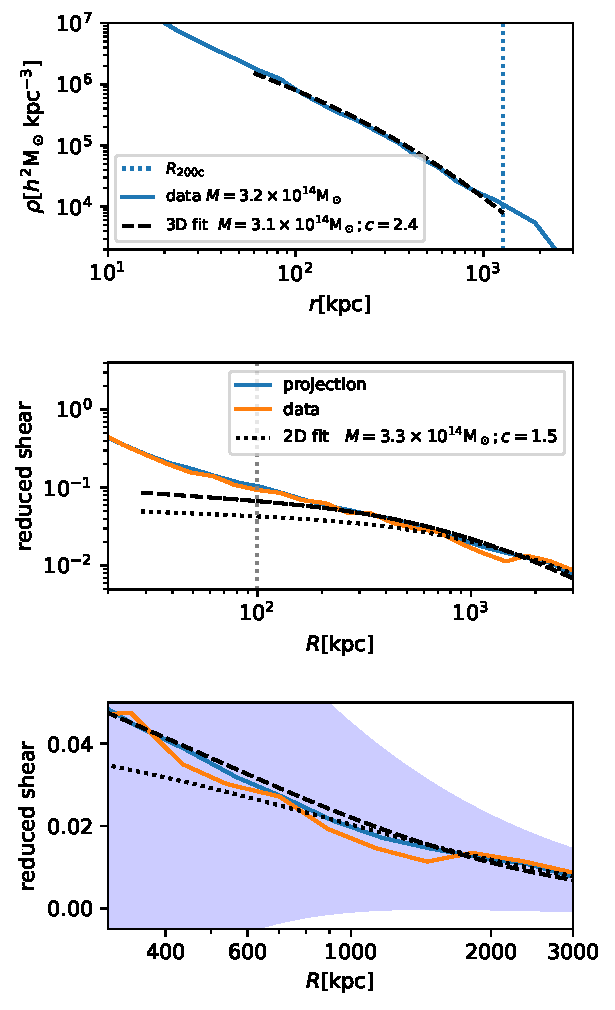
\includegraphics{figure/check_fit_slope1.pdf}}
\caption[h]{Density profiles of a simulated halo and the corresponding  NFW fits. Upper panel: total matter density profile (blue solid line) and the respective NFW fit profile (black dashed line). Central panel: reduced shear from simulated particles (orange solid line), and from the analytical projection of the density profile $\Sigma_{\rm conv.}$ presented in Eq. \eqref{eq:sigmaconv} and performed in the radial range $[60,3000]\,{\rm kpc}$, in the blue solid line. The dashed vertical line indicates the minimum radius of the shear fit, and the fit profiles (black lines) are extrapolated down to $10\,{\rm kpc}$ to enhance the central densities predicted by the two fits. Bottom panel shows the same as central panel but focused in the radial range of the fit. Shaded area reports the uncertainty in the reduced shear as defined in Eq. \eqref{eq:deltag}.}
\label{fig:example}
\end{figure}




\begin{figure}
\scalebox{.85}{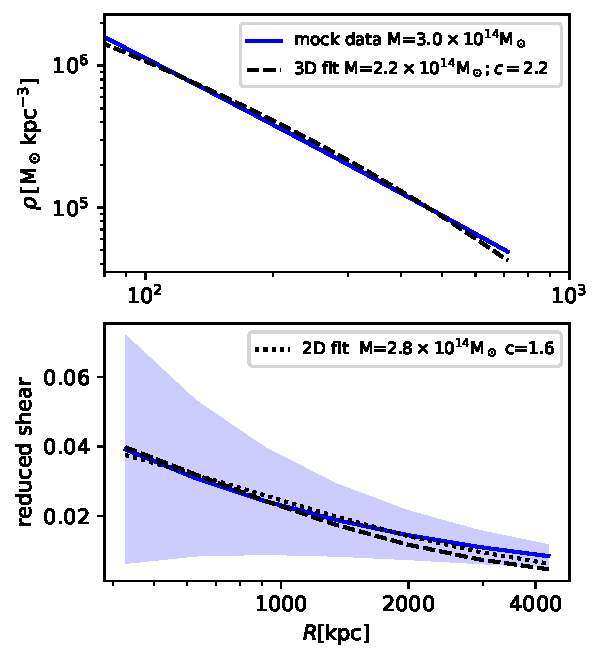
\includegraphics{figure/fit_colossus.pdf}}
\caption[h]{
Density profiles of a mock halo that deviates from NFW and the corresponding  NFW fits.
The mock halo mass, concentration parameter and gNFW log-slopes are chosen to match the ones of the simulated halo presented in Fig.\,\ref{fig:example}.
Upper panel reports the total matter density profile density profile of the mock halo (solid blue line) and the profile from the corrsponding NFW fit (dashed black line). Bottom panel shows the reduced shear and the profile from the corresponding NFW fit (dotted black line). 
 Shaded area reports the uncertainty in the reduced shear as defined in Eq. \eqref{eq:deltag}.}
\label{fig:colossus}
\end{figure}



\section{Correlations with different overdensities}
\label{ap:500}


\iffalse
\begin{figure}
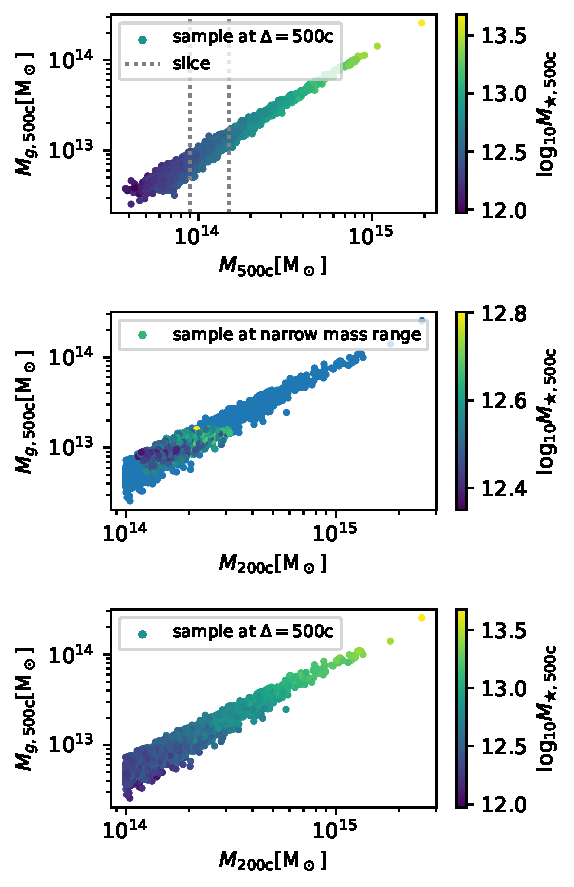
\includegraphics[width=\linewidth]{figure/Mstar_500c_vs_200c.pdf}
\caption[h]{Gas mass, colour coded as stellar mass, both within $r_{\rm 500c}$ as a function of different overdensities. Top panel shows the two quantities as a function $M_{\rm 200c},$ together with a narrow mass bin delimiter around $10^{14}{\rm M}_\odot.$ 
The central panel shows the complete sample as a function of $M_{\rm 200c}$ (blue points) and the coloured points that were selected in the narrow bin in the top panel. The bottom panel shows the complete sample as a function of $M_{\rm 200c}.$
}
\label{fig:500_vs_200}
\end{figure}

To show this point more clearly, in the top panel Fig.\,\ref{fig:500_vs_200} we show for instance the gas mass colour coded by stellar mass, both within $r_{\rm 500c}$ as a function of $M_{\rm 500c}.$ We can see that there is a slight anti-correlation between the two quantities (see darker points are on the upper part of the relation.
If we take a narrow mass bin around $M_{\rm 500c}$ (e.g., one around $10^{14}\,{\rm M}_\odot$ as marked the top panel) and convert to  $M_{\rm 500c},$ as shown in the middle panel, we can see that points will spread without keeping the same anti-correlation found in the first panel.


Therefore when translating the gas and stellar mass correlation within $r_{\rm 500c}$ from $M_{\rm 500c}$ to $M_{\rm 200c},$ as presented in the bottom panel of the Fig. ~\ref{fig:500_vs_200} we see that the two shows a different correlation than before.
As a consequence, having abscissa and ordinate quantities with two different overdensity will bring an additional correlations.
\fi

\begin{figure}
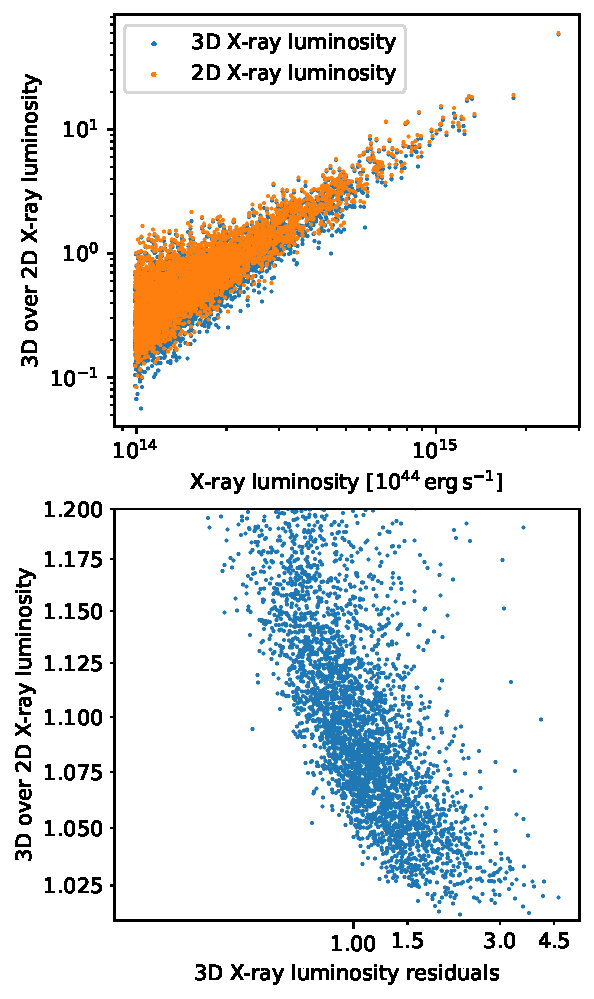
\includegraphics[width=\linewidth]{figure/Xray_scatter_3D_vs_2D.pdf}
\caption[h]{Projected and 3D bolometric X-ray luminosities within $r_{\rm 500c}.$ Top panel shows a scatter plot of the two mass-observable relations, while the bottom panel shows their ratio as a function of the 3D X-ray scaling relation residuals.}
\label{fig:LX3D_vs_2D}
\end{figure}

\begin{figure}
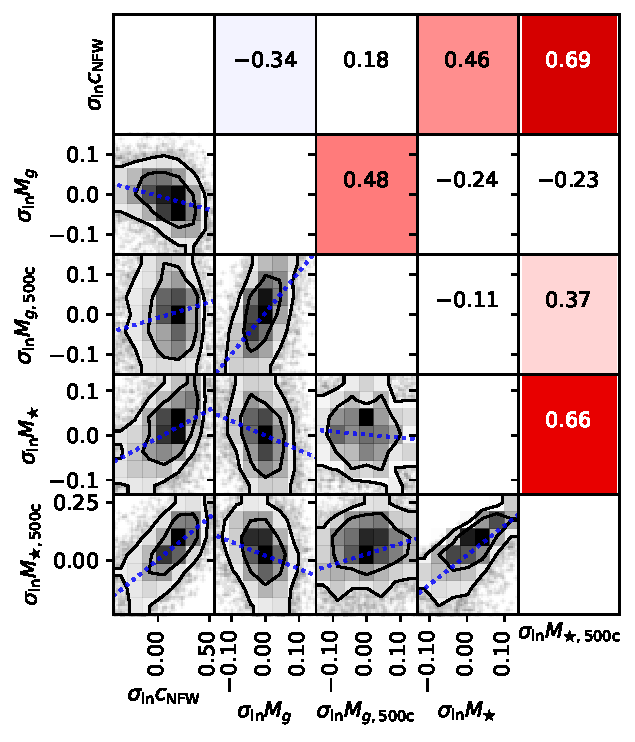
\includegraphics[width=\linewidth]{figure/covarma_500_vs_200.pdf}
\caption[h]{We report the correlation coefficient between concentration, gas mass and stellar mass computed at both $r_{\rm 500c}$ and $r_{\rm 200c}.$}
\label{fig:covarma_500_vs_200}
\end{figure}

In this appendix we discuss the differences between scaling relation scatters and covariance values at different overdensities. 
First of all we tackle the fact that, when we compute X-ray luminosity within $r_{\rm 500c}$ (instead of $r_{\rm 200c}$) we find that the scatter of the scaling relation of the projected quantity is larger than the 3D one.

To investigate this feature, we will focus on the bolometric X-ray luminosity. We report the 3D and projected bolometric X-ray luminosity in Fig. ~\ref{fig:LX3D_vs_2D} (top panel) where it visually clear that the projected X-ray luminosity is (as expected) always larger than the 3D one. One can also notice that the increase in X-ray luminosity depends on the fact that a halo is over-luminous or not: thhe increase of luminosity groin from the 3D to 2D is larger for under-luminous haloes than for over-luminous haloes. We prove this point in the bottom panel of Fig. ~\ref{fig:LX3D_vs_2D} where we show the ratio between the 2D and 3D luminosity as a function of their residual of the 3D scaling relation (the higher the value of the x axis, the more over-luminous is the object for its mass bin), where we can see a strong anti-correlation: overly luminous objects (for a given mass bin) are not going to be affected much by the fact that their luminosity is computed in 3D or 2D. The possible cause is that an interloper in the LoS will not affect much an overly luminous object.  

For completeness, in Fig.\,\ref{fig:covarma_500_vs_200} we show the correlation coefficients between the gas mass and stellar mass computed within both $r_{\rm 500c}$ and $r_{\rm 200c}$ and the concentration.
Here we can see a change of sign on the between $M_{\star,\rm 500c}$-$M_{g,\rm 500c}$ correlations and $M_{\star,\rm 500c}$-$M_{\rm g}$ correlations and a change in the sign between $c_{\rm NFW}$-$M_{\rm g}$ correlations and $c_{\rm NFW}$-$M_{g,\rm500c}$  correlations.

\begin{figure*}
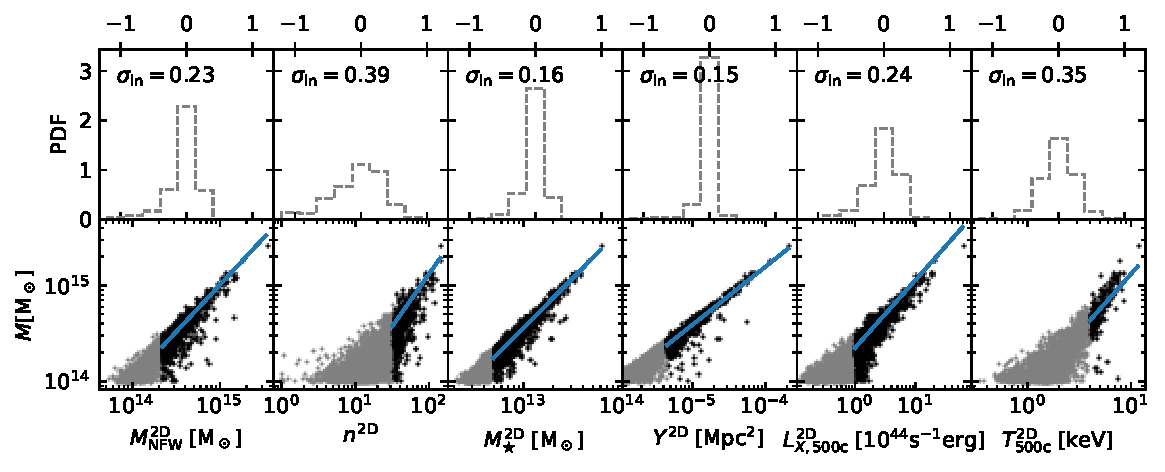
\includegraphics[width=\linewidth]{figure/obs_scatter.pdf}
\caption[h]{Halo masses at fixed observable properties.
We report the  lensing mass, lensing richness, projected stellar mass, projected integrated Compton-$y$, projected X-ray luminosity,  and projected temperature in each column respectively. Top panel shows residuals of the observable-mass relations and respective scatter of log-residuals $\sigma_{\rm ln},$ and its axes are on the upper part of the plot. The bottom panel shows the scaling relation fit (blue solid line), the data used to perform the fit (black data points) over-plotted on top of the total sample (gray data points) of the mass $M$ as a function of the observable properties. 
}
\label{fig:obs_scatter}
\end{figure*}



Finally, in Fig.\,\ref{fig:obs_scatter} we report the scatter of observable properties at fixed mass for both \Euclid-like quantities (lensing mass, richness, and projected stellar mass), and possible multi wavelength properties (integrated Compton-$y$ and X-ray luminosity, temperature), where we compute X-ray luminosity and temperature within $r_{\rm 500c}$ as they are typically derived within this overdensity.
The upper panel of Fig.\,\ref{fig:obs_scatter} shows the residuals of the log-log linear regression where we see that in terms of 2D scatter, the properties with lowest scatter are the stellar mass and the temperature.
The bottom panel shows the data points used to perform the fit (in black) where we used a visually-inspected cut on the halo mass values in order to ensure that mass values are complete for a given observable value. 

\begin{table*}
\caption{Scatter and correlation coefficient matrix between $z=0.24$ log-residuals of scaling relations.}              % title of Table
\label{table:z0}      % is used to refer this table in the text
\centering   % used for centering table
\small
\setlength\tabcolsep{1.4pt}
\begin{tabular}{l  r  r  r  r  r  r  r  r  r  r  r  r  r  r  r  r  r  r  r  r  r }
 \hline\hline & 
$c_{\rm NFW}$ & $M^{\rm 2D}_{\rm NFW}$ & $n$ & $n^{\rm 2D}$ & $M_{\bigstar}$ & $M_{\bigstar}^{\rm 2D}$ & $Y$ & $Y^{\rm 2D}$ & $M_{\rm g}$ & $M_{\rm g}^{\rm 2D}$ & $M_{g,{\rm 500c}}$ & $M^{\rm 2D}_{g,{\rm 500c}}$ & $L_X$ & $L_X^{\rm 2D}$ & $L_{X,{\rm 500c}}$ & $L^{\rm 2D}_{X,{\rm 500c}}$ & $L^{\rm 2D}_{X,ce{\rm 500c}}$ & $T$ & $T^{\rm 2D}$ & $T_{\rm 500c}$ & $T^{\rm 2D}_{\rm 500c}$ \\ \hline   
$c_{\rm NFW}$ &  $0.31$&         &         &         &         &         &         &         &         &         &         &         &         &         &         &         &         &         &         &         &          \\ 
$M^{\rm 2D}_{\rm NFW}$ &  $0.25$& $0.24$&         &         &         &         &         &         &         &         &         &         &         &         &         &         &         &         &         &         &          \\ 
$n$ & $-0.27$&   $--$  & $0.26$&         &         &         &         &         &         &         &         &         &         &         &         &         &         &         &         &         &          \\ 
$n^{\rm 2D}$ & $-0.19$& $0.33$& $0.70$& $0.31$&         &         &         &         &         &         &         &         &         &         &         &         &         &         &         &         &          \\ 
$M_{\bigstar}$ &  $0.36$&   $--$  &   $--$  &   $--$  & $0.08$&         &         &         &         &         &         &         &         &         &         &         &         &         &         &         &          \\ 
$M_{\bigstar}^{\rm 2D}$ &    $--$  & $0.57$&   $--$  & $0.57$& $0.48$& $0.15$&         &         &         &         &         &         &         &         &         &         &         &         &         &         &          \\ 
$Y$ &  $0.33$&   $--$  &$-0.23$&   $--$  &   $--$  &   $--$  & $0.08$&         &         &         &         &         &         &         &         &         &         &         &         &         &          \\ 
$Y^{\rm 2D}$ &    $--$  & $0.46$&   $--$  & $0.32$&   $--$  & $0.64$& $0.39$& $0.17$&         &         &         &         &         &         &         &         &         &         &         &         &          \\ 
$M_{\rm g}$ & $-0.28$&   $--$  & $0.23$& $0.20$&$-0.29$&   $--$  & $0.39$&   $--$  & $0.04$&         &         &         &         &         &         &         &         &         &         &         &          \\ 
$M_{\rm g}^{\rm 2D}$ &    $--$  & $0.56$&   $--$  & $0.53$&   $--$  & $0.71$&   $--$  & $0.79$&   $--$  & $0.20$&         &         &         &         &         &         &         &         &         &         &          \\ 
$M_{g,{\rm 500c}}$ &    $--$  &   $--$  &   $--$  &   $--$  &$-0.28$&$-0.24$& $0.53$&   $--$  & $0.45$&   $--$  & $0.15$&         &         &         &         &         &         &         &         &         &          \\ 
$M^{\rm 2D}_{g,{\rm 500c}}$ &    $--$  & $0.60$&   $--$  & $0.50$&   $--$  & $0.67$&   $--$  & $0.76$&   $--$  & $0.96$&   $--$  & $0.18$&         &         &         &         &         &         &         &         &          \\ 
$L_X$ & $-0.20$&   $--$  & $0.25$&   $--$  &$-0.20$&   $--$  &   $--$  &   $--$  & $0.52$&   $--$  & $0.52$&   $--$  & $0.24$&         &         &         &         &         &         &         &          \\ 
$L_X^{\rm 2D}$ &    $--$  & $0.31$& $0.26$& $0.48$&   $--$  & $0.32$&   $--$  & $0.23$& $0.45$& $0.39$& $0.36$& $0.44$& $0.78$& $0.27$&         &         &         &         &         &         &          \\ 
$L_{X,{\rm 500c}}$ &    $--$  &   $--$  &   $--$  &   $--$  &$-0.19$&   $--$  & $0.33$&   $--$  & $0.45$&   $--$  & $0.74$&   $--$  & $0.90$& $0.67$& $0.30$&         &         &         &         &         &          \\ 
$L^{\rm 2D}_{X,{\rm 500c}}$ &    $--$  & $0.20$& $0.21$& $0.28$&$-0.23$&   $--$  & $0.24$&   $--$  & $0.50$&   $--$  & $0.59$& $0.22$& $0.87$& $0.87$& $0.87$& $0.28$&         &         &         &         &          \\ 
$L^{\rm 2D}_{X,ce{\rm 500c}}$ & $-0.31$&   $--$  & $0.20$& $0.29$&$-0.29$&   $--$  &   $--$  &   $--$  & $0.49$&   $--$  & $0.59$& $0.24$& $0.69$& $0.75$& $0.65$& $0.85$& $0.31$&         &         &         &          \\ 
$T$ &  $0.52$& $0.20$&$-0.23$&   $--$  &   $--$  &   $--$  & $0.54$&   $--$  &   $--$  &   $--$  & $0.34$&   $--$  &   $--$  &   $--$  &   $--$  &   $--$  &   $--$  & $0.22$&         &         &          \\ 
$T^{\rm 2D}$ &  $0.47$&   $--$  &$-0.22$&$-0.29$&   $--$  &   $--$  & $0.51$&   $--$  &   $--$  &$-0.20$& $0.37$&   $--$  &   $--$  &$-0.25$&   $--$  &   $--$  &   $--$  & $0.91$& $0.24$&         &          \\ 
$T_{\rm 500c}$ &  $0.52$& $0.20$&$-0.22$&   $--$  &   $--$  &   $--$  & $0.46$&   $--$  &   $--$  &   $--$  & $0.23$&   $--$  &   $--$  &   $--$  &   $--$  &   $--$  &   $--$  & $0.95$& $0.85$& $0.22$&          \\ 
$T^{\rm 2D}_{\rm 500c}$ &  $0.48$&   $--$  &$-0.21$&$-0.28$&   $--$  &   $--$  & $0.50$&   $--$  &   $--$  &$-0.20$& $0.34$&   $--$  &   $--$  &$-0.25$&   $--$  &   $--$  &   $--$  & $0.91$& $0.98$& $0.87$& $0.23$ \\ 
\hline\end{tabular}
\tablefoot{Diagonal terms report the  scatter of the log-residuals of each quantity, namely $\sigma_{\rm ln}$ of Eq.~\eqref{eq:sigmaln}, while the off-diagonal terms report the correlation coefficient between the log-residuals. We do not report values of the correlation coefficient below $0.20$ because they are not significant. We do not report the values for the 3D NFW mass $M_{\rm 200c}$ because it has a very low scatter of log-residuals ($\approx0.01$) and its correlation coefficients are not meaningful.
Note that in this table we also added the core-excised X-ray luminosity.}
\end{table*}

 \begin{table*}
\caption{Scatter and correlation coefficient matrix between $z=0.9$ log-residuals of scaling relations.}              % title of Table
\label{table:z1}      % is used to refer this table in the text
\centering   % used for centering table
\small
\setlength\tabcolsep{1.4pt}
\begin{tabular}{l  r  r  r  r  r  r  r  r  r  r  r  r  r  r  r  r  r  r  r  r  r }
 \hline\hline & 
$c_{\rm NFW}$ & $M^{\rm 2D}_{\rm NFW}$ & $n$ & $n^{\rm 2D}$ & $M_{\bigstar}$ & $M_{\bigstar}^{\rm 2D}$ & $Y$ & $Y^{\rm 2D}$ & $M_{\rm g}$ & $M_{\rm g}^{\rm 2D}$ & $M_{g,{\rm 500c}}$ & $M^{\rm 2D}_{g,{\rm 500c}}$ & $L_X$ & $L_X^{\rm 2D}$ & $L_{X,{\rm 500c}}$ & $L^{\rm 2D}_{X,{\rm 500c}}$ & $L^{\rm 2D}_{X,ce{\rm 500c}}$ & $T$ & $T^{\rm 2D}$ & $T_{\rm 500c}$ & $T^{\rm 2D}_{\rm 500c}$ \\ \hline   
$c_{\rm NFW}$ &  $0.32$&         &         &         &         &         &         &         &         &         &         &         &         &         &         &         &         &         &         &         &          \\ 
$M^{\rm 2D}_{\rm NFW}$ &  $0.24$& $0.24$&         &         &         &         &         &         &         &         &         &         &         &         &         &         &         &         &         &         &          \\ 
$n$ & $-0.29$&   $--$  & $0.26$&         &         &         &         &         &         &         &         &         &         &         &         &         &         &         &         &         &          \\ 
$n^{\rm 2D}$ & $-0.22$& $0.36$& $0.70$& $0.31$&         &         &         &         &         &         &         &         &         &         &         &         &         &         &         &         &          \\ 
$M_{\bigstar}$ &  $0.37$&   $--$  &   $--$  &   $--$  & $0.08$&         &         &         &         &         &         &         &         &         &         &         &         &         &         &         &          \\ 
$M_{\bigstar}^{\rm 2D}$ &    $--$  & $0.60$&   $--$  & $0.55$& $0.48$& $0.15$&         &         &         &         &         &         &         &         &         &         &         &         &         &         &          \\ 
$Y$ &  $0.34$&   $--$  &$-0.23$&   $--$  &   $--$  &   $--$  & $0.08$&         &         &         &         &         &         &         &         &         &         &         &         &         &          \\ 
$Y^{\rm 2D}$ &    $--$  & $0.46$&   $--$  & $0.31$&   $--$  & $0.63$& $0.40$& $0.17$&         &         &         &         &         &         &         &         &         &         &         &         &          \\ 
$M_{\rm g}$ & $-0.29$&   $--$  & $0.23$& $0.21$&$-0.30$&   $--$  & $0.39$&   $--$  & $0.05$&         &         &         &         &         &         &         &         &         &         &         &          \\ 
$M_{\rm g}^{\rm 2D}$ &    $--$  & $0.58$&   $--$  & $0.52$&   $--$  & $0.70$&   $--$  & $0.79$&   $--$  & $0.20$&         &         &         &         &         &         &         &         &         &         &          \\ 
$M_{g,{\rm 500c}}$ &    $--$  &   $--$  &   $--$  &   $--$  &$-0.28$&$-0.25$& $0.52$&   $--$  & $0.45$&   $--$  & $0.15$&         &         &         &         &         &         &         &         &         &          \\ 
$M^{\rm 2D}_{g,{\rm 500c}}$ &    $--$  & $0.63$&   $--$  & $0.49$&   $--$  & $0.66$&   $--$  & $0.76$&   $--$  & $0.96$&   $--$  & $0.18$&         &         &         &         &         &         &         &         &          \\ 
$L_X$ & $-0.20$&   $--$  & $0.26$&   $--$  &$-0.20$&   $--$  &   $--$  &   $--$  & $0.52$&   $--$  & $0.50$&   $--$  & $0.25$&         &         &         &         &         &         &         &          \\ 
$L_X^{\rm 2D}$ & $-0.19$& $0.34$& $0.26$& $0.48$&   $--$  & $0.31$&   $--$  & $0.22$& $0.44$& $0.39$& $0.35$& $0.44$& $0.78$& $0.28$&         &         &         &         &         &         &          \\ 
$L_{X,{\rm 500c}}$ &    $--$  &   $--$  &   $--$  &   $--$  &$-0.20$&   $--$  & $0.33$&   $--$  & $0.46$&   $--$  & $0.73$&   $--$  & $0.89$& $0.67$& $0.30$&         &         &         &         &         &          \\ 
$L^{\rm 2D}_{X,{\rm 500c}}$ &    $--$  & $0.23$& $0.22$& $0.29$&$-0.24$&   $--$  & $0.23$&   $--$  & $0.50$&   $--$  & $0.58$& $0.22$& $0.87$& $0.86$& $0.87$& $0.28$&         &         &         &         &          \\ 
$L^{\rm 2D}_{X,ce{\rm 500c}}$ & $-0.31$& $0.22$& $0.22$& $0.31$&$-0.30$&   $--$  &   $--$  &   $--$  & $0.50$&   $--$  & $0.58$& $0.23$& $0.69$& $0.74$& $0.65$& $0.85$& $0.31$&         &         &         &          \\ 
$T$ &  $0.51$&   $--$  &$-0.22$&   $--$  &   $--$  &   $--$  & $0.52$&   $--$  &   $--$  &   $--$  & $0.33$&   $--$  &   $--$  &   $--$  &   $--$  &   $--$  &   $--$  & $0.22$&         &         &          \\ 
$T^{\rm 2D}$ &  $0.46$&   $--$  &$-0.22$&$-0.29$&   $--$  &   $--$  & $0.50$&   $--$  &   $--$  &$-0.21$& $0.36$&   $--$  &   $--$  &$-0.28$&   $--$  &   $--$  &   $--$  & $0.90$& $0.24$&         &          \\ 
$T_{\rm 500c}$ &  $0.52$&   $--$  &$-0.21$&   $--$  &   $--$  &   $--$  & $0.45$&   $--$  &   $--$  &   $--$  & $0.21$&   $--$  &$-0.20$&   $--$  &   $--$  &   $--$  &   $--$  & $0.95$& $0.84$& $0.22$&          \\ 
$T^{\rm 2D}_{\rm 500c}$ &  $0.48$&   $--$  &$-0.21$&$-0.28$&   $--$  &   $--$  & $0.49$&   $--$  &   $--$  &$-0.20$& $0.34$&   $--$  &   $--$  &$-0.28$&   $--$  &   $--$  &   $--$  & $0.90$& $0.98$& $0.87$& $0.24$ \\ 
\hline\end{tabular}
\tablefoot{Rows and columns are as in Table~\ref{table:z0}. We do not present the lensing concentration $c_{\rm NFW}^{\rm 2D}$ because the radial range  of the reduced shear fit that we used at this redshift is not able to capture the concentration.}
\end{table*}
 \end{appendix}
\end{document}
